\documentclass[10pt,a4paper,openany]{memoir}
\makeatletter
\createmark{chapter}{both}{shownumber}{\@chapapp\ }{. \ }
\makeatother
\makeheadrule{headings}{\textwidth}{0.3pt}
\makeevenfoot{headings}{\thepage}{}{}
\makeoddfoot{headings}{}{}{\thepage}
\makeoddhead{headings}{}{}{\rightmark}
\makeevenhead{headings}{\leftmark}{}{}
\makeevenfoot{plain}{\thepage}{}{}
\makeoddfoot{plain}{}{}{\thepage}
\clearmark{section}
\setsecnumdepth{subsection}
\usepackage{siunitx}
\usepackage{overcite}
\usepackage{microtype}
\usepackage[utf8]{inputenc}
\usepackage{amsmath}
\usepackage{amsfonts}
\usepackage{booktabs}
\usepackage{longtable}
\usepackage{amssymb}
\usepackage{graphicx}
\usepackage{listings}
\usepackage{lmodern}
\usepackage{gensymb}
\usepackage{hyperref}
\usepackage{lscape}
\numberwithin{equation}{section}
\def\chapterautorefname{Chapter}
\def\sectionautorefname{Section}
\def\subsectionautorefname{Section}
\def\pageautorefname{p.}
\DeclareMathOperator{\sign}{sign}
\renewcommand*{\thefootnote}{\fnsymbol{footnote}}
\newcommand{\under}{\_}
\newcommand{\rsub}[1]{\mathbf{r}_{#1}}
\newcommand{\fsub}[1]{\mathbf{f}_{#1}}
\newcommand{\ssub}[1]{\mathbf{s}_{#1}}
\newcommand{\revyan}[1]{{\color{red}{[#1]}}}
\newcommand{\profileropt}[0]{\texttt{profilerOpt}}
\newcommand{\profilergen}[0]{\texttt{profilerGen}}
\newcommand{\profilertools}[0]{\texttt{profilerTools}}
\usepackage[left=.75in,right=.75in,top=.5in,bottom=.75in]{geometry}
\newcommand{\varset}[2]{$\text{#1}=#2$}
\usepackage{color}

\definecolor{mygreen}{rgb}{0,0.6,0}
\definecolor{mygray}{rgb}{0.85,0.85,0.85}
\definecolor{mymauve}{rgb}{0.58,0,0.82}

% \setlength{\droptitle}{50pt}
\renewcommand{\maketitlehooka}{%
  \vfill\hrulefill}
\renewcommand{\maketitlehookb}{%
  \hrulefill\par \hfill \textit{Corresponding to Version 1.0}}
\renewcommand{\maketitlehookc}{%
  \vfill}
\title{\Huge\texttt{profilerTools} \\ User Manual}
\author{{\huge MSSM Group} \\ Maintained by Yan M. H. Gonçalves}
\date{\footnotesize\textcopyright 2020--: \hspace{5ex}
  MSSM Group, Laboratório de Modelagem Molecular,\\
  \hspace{16ex} Instituto de Química, Universidade Federal do Rio de Janeiro}
  
\lstdefinelanguage{gromacs}{morecomment=[l]{;}}
\lstset{
  backgroundcolor=\color{mygray},   % choose the background color; you must add \usepackage{color} or \usepackage{xcolor}; should come as last argument
  basicstyle=\footnotesize\ttfamily,        % the size of the fonts that are used for the code
  breakatwhitespace=false,         % sets if automatic breaks should only happen at whitespace
  belowskip=-4pt,
    aboveskip=-4pt,
  breaklines=true,                 % sets automatic line breaking
  captionpos=b,                    % sets the caption-position to bottom
  commentstyle=\color{mygreen},    % comment style
  deletekeywords={...},            % if you want to delete keywords from the given language
  escapeinside={\%*}{*)},          % if you want to add LaTeX within your code
  extendedchars=true,              % lets you use non-ASCII characters; for 8-bits encodings only, does not work with UTF-8
  firstnumber=01,                % start line enumeration with line 1000
  frame=single,	                   % adds a frame around the code
  keepspaces=true,                 % keeps spaces in text, useful for keeping indentation of code (possibly needs columns=flexible)
%  keywordstyle=\color{blue},       % keyword style
  language=Bash,                 % the language of the code
  morekeywords={*,...},            % if you want to add more keywords to the set
  numbers=none,                    % where to put the line-numbers; possible values are (none, left, right)
  numbersep=5pt,                   % how far the line-numbers are from the code
  numberstyle=\tiny\color{mygray}, % the style that is used for the line-numbers
  rulecolor=\color{white},         % if not set, the frame-color may be changed on line-breaks within not-black text (e.g. comments (green here))
  showspaces=false,                % show spaces everywhere adding particular underscores; it overrides 'showstringspaces'
  showstringspaces=false,          % underline spaces within strings only
  showtabs=false,                  % show tabs within strings adding particular underscores
  stepnumber=1,                    % the step between two line-numbers. If it's 1, each line will be numbered
  stringstyle=\color{mymauve},     % string literal style
  tabsize=4,	                   % sets default tabsize to 2 spaces
  columns=fullflexible,  
  title=\lstname                   % show the filename of files included with \lstinputlisting; also try caption instead of title
}

\lstdefinestyle{ascii-tree}{
    literate={├}{|}1 {─}{--}1 {└}{+}1 
  }

  \begin{document}
  \maketitle
  \thispagestyle{empty}

  \clearpage
  \frontmatter
  \nouppercaseheads
  \addtolength{\headheight}{2ex}
  \addtolength{\headsep}{-2ex}

  \section{Citation Information}

  % If the \profilertools{} suite was helpful in achieving your results,
  % we kindly ask you to cite the following paper:

  % \begin{quote}
  %   Long title of the paper, with many things. Many details of the
  %   journal, such as name and pages. Possibly also a DOI: xxxxxxx.
  % \end{quote}

  % \noindent If you wish to cite this manual, please refer to it as

  % \begin{quote}
  %   Gonçalves, Y.~M.~H. \textit{profilerTools: User Manual
  %   (v1.0)}. \url{https://github.com/mssm-labmmol/profiler} (2020).
  % \end{quote}

  In the absence of a scientific publication, we kindly ask you to
  cite this manual if the \profilertools{} suite was helpful in
  achieving your results, referring to it as

  \begin{quote}
    Gonçalves, Y.~M.~H. and the MSSM Group. \textit{profilerTools: User Manual
      (Version 1.0)}.\\
    \url{https://github.com/mssm-labmmol/profiler}
    (2020).
  \end{quote}

  \section{License}

  \profilertools{} is released under the MIT License. For more
  information, check the LICENSE file supplied with the source code or
  consult \autoref{appendix:MIT-license}

  \section{Contact}

  For bug reports or other software-related questions, send an e-mail
  to \url{yanmarques@gmail.com}.  More information about our research
  group can be found on the webpage
  \url{https://labmmol.iq.ufrj.br/mssm}.

\tableofcontents

  \mainmatter

\newcommand*{\profi}{\texttt{profilerOpt}}

\chapter{Introduction}
\label{chap:intro}

Dihedral-angle torsion parameters are typically optimized using
quantum-mechanical relative conformational energies as target data.
%
However, confomational energies are also affected by the 1,4 nonbonded
interactions.
%
This suggests that these two types of force-field terms should ideally
be parameterized simultaneously.
%
With that in mind, we developed \profileropt{}, a Python program that
allows this by means of an evolutionary-computing-driven
optimization.
%
As usual, the optimization is based on the reproduction of relative
conformational energies, also supporting the use of reference data for
several molecules at once.
%
Together with \profilergen{}, an auxiliary Python program to execute
multidimensional molecular torsional scans, these two form the
\profilertools{} suite.
%

More succinctly, \profilertools{} is composed of two programs:

\begin{itemize}
\item \profilergen, for obtaining torsional-scan trajectories and
  their energy profiles;
\item \profileropt, for the parameterization of torsional terms and
  the related 1,4 Lennard-Jones terms;
\end{itemize}

The evolutionary algorithms are based on the DEAP library\cite{DEAP}.
Two of them are implemented in \profilertools{}: genetic algorithms
(GAs) and covariance matrix adaptation evolution strategy (CMA-ES).

Another important feature of \profilertools{} is that it does not rely
on external libraries for carrying out molecular-mechanics
calculations and energy minimizations. The mathematical formluae and
the supported physical models are described in \autoref{chap:mm}. They
are implemented based on \texttt{numpy} and on a \texttt{C} extension
to \texttt{numpy} called \texttt{geometrypy}, specifically implemented
for \profilertools. This extension accelerates the calculation of
geometric degrees of freedom (bond lengths, bond-angle angles, etc.)
by transferring the loops over the involved atoms to the underlying
\texttt{C} implementation, instead of carrying out these loops in
Python (which is significantly slower).


\chapter{Molecular Mechanics and Energy Minimization}
\label{chap:mm}

In \profilertools{}, molecular-mechanics energies and forces are
calculated using custom code which depends only on standard Python
libraries and \texttt{numpy}.
%
In this chapter, we give details about the computation of all quantities which directly involve these calculations.
First, we report all force-field functional forms available in the suite.
After that, we give the expressions for the calculation of forces.
We then describe the energy minimization algorithms implemented in the programs.
Finally, we define the central object of the molecular-mechanics calculations of \profilertools{}, namely, the torsional scan and its corresponding energy profile.

Considering a system of $N$ particles, the following notation and definitions will be used for mathematical and physical quantities whenever convenient:

\begin{itemize}
\item[---] $\mathbf{u} \cdot \mathbf{v}$ \par  Dot product of vectors $\mathbf{u}$ and $\mathbf{v}$.
\item[---] $\mathbf{u} \times \mathbf{v}$ \par  Cross product of vectors $\mathbf{u}$ and $\mathbf{v}$.
\item[---] $\mathbf{r}_i$ \par  Position of particle $i$.
\item[---] $\mathbf{r}_{ij} = \mathbf{r}_i - \mathbf{r}_j$ \par  Displacement from particle $j$ to particle $i$.
\item[---] $r_{ij} = \sqrt{\mathbf{r}_{ij} \cdot \mathbf{r}_{ij}}$ \par  Distance between particle $i$ and particle $j$.
\item[---] $\theta_{ijk} = \arccos{\frac{\mathbf{r}_{ij} \cdot \mathbf{r}_{kj}}{r_{ij}r_{kj}}}$  \par  Angle involving particles $i$, $j$ and $k$.
\item[---] $\phi_{ijkl} = \sign{(\rsub{ij} \cdot \rsub{nk})} \arccos{\left( \frac{\rsub{mj} \cdot \rsub{nk}}{r_{mj}r_{nk}} \right)}$, with $\rsub{mj} = \rsub{ij}\times\rsub{kj}$ and $\rsub{nk} = \rsub{kj}\times\rsub{kl}$
  \par  Dihedral angle involving particles $i$, $j$, $k$ and $l$.
\item[---] $\mathbf{r}(t_n) = (\rsub{1}(t_n),\rsub{2}(t_n)\ldots\rsub{N}(t_n))$
  \par
  
  Configuration at the $n$-th step of the energy-minimization algorithm.
\item[---] $\mathbf{f}(t_n) = (\fsub{1}(t_n),\fsub{2}(t_n)\ldots\fsub{N}(t_n))$
  \par
  Configuration of the forces at the $n$-th step of the energy-minimization~algorithm.
\end{itemize}

\section{Force-field Functional Forms}
\label{sec:mm-force-field-functional-forms}


\subsection{Bond stretching}
\label{sec:bond-terms}

The following functional forms are supported for the calculation of
the energies and forces associated with a bond-stretching degree of freedom:\cite{GROMOS-doc,GROMACS-doc}

\begin{itemize}
\item [---] \textit{Harmonic}
  \par
  Potential energy form:
  \begin{align}
    \label{eq:harmonic-bond-energy}
    V(r_{ij}; k_b^h, b_0) & = \frac{1}{2} \ k_b^h (r_{ij} - b_0)^2 \quad , \\ \nonumber
    \frac{\partial V(r_{ij}; k_b^h, b_0)}{\partial r_{ij}} & = \ k_b^h (r_{ij} - b_0) \quad ,
  \end{align}
  
\item [---] \textit{Quartic}
  \par
  Potential energy form:
  \begin{align}
    \label{eq:quartic-bond-energy}
    V(r_{ij}; k_b^q, b_0) & = \frac{1}{4} \ k_b^q (r_{ij}^2 - b_0^2)^2 \quad , \\ \nonumber
    \frac{\partial V(r_{ij}; k_b^q, b_0)}{\partial r_{ij}} & = r_{ij} k_b^q (r_{ij}^2 - b_0^2) \quad ,
  \end{align}

\end{itemize}

\noindent
where $V(r_{ij})$ is the potential energy term for the bond between particles $i$ and $j$.

\subsection{Bond-angle stretching}
\label{sec:angle-terms}

The following functional forms are supported for the calculation of
the energies and forces associated with a bond-angle stretching degree of freedom:\cite{GROMOS-doc,GROMACS-doc}

\begin{itemize}
\item [---] \textit{Harmonic}
  \par
  Potential energy form:
  \begin{align}
    \label{eq:harmonic-angle-energy}
    V(\theta_{ijk}; k_a^h, \theta_0) & = \frac{1}{2} \ k_a^h (\theta_{ijk} - \theta_0)^2 \quad , \\ \nonumber
    \frac{\partial V(\theta_{ijk}; k_a^h, \theta_0)}{\theta_{ijk}} & = k_a^h (\theta_{ijk} - \theta_0) \quad ,
  \end{align}
  
\item [---] \textit{Cosine-harmonic}
  \par
  Potential energy form:
  \begin{align}
    \label{eq:cosine-angle-energy}
    V(\theta_{ijk}; k_a^c, \theta_0) & = \frac{1}{2} \ k_a^c (\cos{\theta_{ijk}} - \cos\theta_0)^2 \quad , \\ \nonumber
    \frac{\partial V(\theta_{ijk}; k_a^c, \theta_0)}{\theta_{ijk}} & = -k_a^c \sin{\theta_{ijk}}(\cos{\theta_{ijk}} - \cos\theta_0) \quad ,
  \end{align}

\item [---] \textit{Urey-Bradley}
  \par
  Potential energy form:
  \begin{align}
    \label{eq:ub-angle-energy}
    V(\theta_{ijk},r_{ik}; k_a^{ub}, \theta_0,k_{13}^{ub},b_{13}^{ub}) & = \frac{1}{2} \ k_a^{ub} (\theta_{ijk} - \theta_0)^2 + \frac{1}{2}  \ k_{13}^{ub} (r_{ik} - b_{13}^{ub})^2 \quad , \\ \nonumber
    \frac{\partial V(\theta_{ijk},r_{ik}; k_a^{ub}, \theta_0,k_{13}^{ub},b_{13}^{ub})}{\partial \theta_{ijk}} & = k_a^{ub} (\theta_{ijk} - \theta_0) \quad , \\ \nonumber
    \frac{\partial V(\theta_{ijk},r_{ik}; k_a^{ub}, \theta_0,k_{13}^{ub},b_{13}^{ub})}{\partial r_{ik}}  & = k_{13}^{ub} (r_{ik} - b_{13}^{ub}) \quad ,
  \end{align}

\end{itemize}  
\noindent
where $V(\theta_{ijk},[r_{ik}])$ is the potential energy term for the angle involving particles $i$, $j$ and $k$.
Note that the Urey-Bradley form introduces dependence on an additional degree of freedom, the distance $r_{ik}$, which is treated as a harmonic bond between particles $i$ and $k$.

\subsection{Proper dihedral-angle torsion}
\label{sec:proper-terms}

The following functional forms are supported for the calculation of
the energies and forces associated with a proper dihedral-angle
torsion degree of freedom:\cite{GROMOS-doc,GROMACS-doc}

\begin{itemize}
\item [---] \textit{Standard periodic}
  \par
  Potential energy form:
  \begin{align}
    \label{eq:proper-standard-energy}
    V(\phi_{ijkl} ; \{k_{d,m}^s, \phi_{0,m}\}_{m=1..6}) & = \sum_{m=1}^{6} k_{d,m}^s\ (1 + \cos{( m \phi_{ijkl} - \phi_{0,m})})\quad , \\ \nonumber
    \frac{\partial V(\phi_{ijkl} ; \{k_{d,m}^s, \phi_{0,m}\}_{m=1..6})}{\partial \phi_{ijkl}} & = -\sum_{m=1}^{6} m k_{d,m}^s \sin{(m \phi_{ijkl} - \phi_{0,m})}\quad ,
  \end{align}
  with $\phi_{0,m} \in (-\pi, \pi]$.
  
\item [---]\textit{Ryckaert-Bellemans}
  \par
  Potential energy form:
  \begin{align}
    \label{eq:proper-rb-energy}
    V(\phi_{ijkl} ; \{c_m\}_{m=0..5}) & = \sum_{m=0}^{5} c_m \cos^m{(\phi_{ijkl}-\pi)} \quad , \\ \nonumber
    \frac{\partial V(\phi_{ijkl} ; \{c_m\}_{m=0..5})}{\partial \phi_{ijkl}} & = \sum_{m=1}^{5} mc_m \sin{\phi_{ijkl}} \cos^{m-1}{(\phi_{ijkl}-\pi)} \quad , 
  \end{align}

\item [---]\textit{Fourier}
  \par
  Potential energy form:
   \begin{align}
    \label{eq:proper-fourier-energy}
     V(\phi_{ijkl} ; \{f_m\}_{m=1..4}) & = \frac{1}{2} \sum_{m=1}^{4} f_m \left[1 + (-1)^{m+1}\cos m\phi_{ijkl}\right] \quad , \\ \nonumber
     \frac{\partial V(\phi_{ijkl} ; \{f_m\}_{m=1..4})}{\partial \phi_{ijkl}} & = \frac{1}{2} \sum_{m=1}^{4} m f_m (-1)^{m}\sin m\phi_{ijkl} \quad ,
   \end{align}
   
   Internally, this potential is computed as a Ryckaert-Bellemans potential with
   \begin{align*}
     c_0 & = f_2 + \frac{1}{2} (f_1 + f_3)\\
     c_1 & = \frac{1}{2} (-f_1 + 3f_3)\\
     c_2 & = -f_2 + 4f_4\\
     c_3 & = -2 f_3\\
     c_4 & = -4 f_4\\
     c_5 & = 0
   \end{align*}

\item [---]\textit{Harmonic restraint}
  \par
  Potential energy form:
  \begin{align}
  \label{eq:proper-restraint-energy}
  V(\phi_{ijkl}; k_d^r, \phi_0) & = \frac{1}{2} k_d^r (\phi_{ijkl} - \phi_0)^2 \quad , \\ \nonumber
  \frac{\partial V(\phi_{ijkl}; k_d^r, \phi_0)}{\partial \phi_{ijkl}} & = k_d^r (\phi_{ijkl} - \phi_0) \quad , 
\end{align}
\end{itemize}
where $V(\phi_{ijkl})$ is the potential energy term for the proper dihedral angle involving particles $i$, $j$, $k$ and $l$.

\subsection{Improper dihedral-angle bending}
\label{sec:improper-terms}

The following functional forms are supported for the calculation of
the energies and forces associated with an improper dihedral-angle
bending degree of freedom:\cite{GROMOS-doc,GROMACS-doc}

\begin{itemize}
\item[---] \textit{Harmonic}
  \par
  Potential energy form:  
\begin{align}
  \label{eq:improper-harmonic-energy}
  V(\phi_{ijkl}; k_i^h, \phi_0) & =  \frac{1}{2} k_i^h (\phi_{ijkl} - \phi_0)^2 \quad , \\ \nonumber
  \frac{\partial V(\phi_{ijkl}; k_i^h, \phi_0)}{\phi_{ijkl}} & = k_i^h (\phi_{ijkl} - \phi_0) \quad ,
\end{align}
\item [---] \textit{Periodic}
  % \par
  % Potential energy form:
  % \begin{align}
  %   \label{eq:improper-periodic-energy}
  %   V(\phi_{ijkl} ; k_{i}^p, \phi_{0}, m) & = k_{i}^p\ (1 + \cos{\phi_{0}} \cos{m \phi_{ijkl}})\quad , \\ \nonumber
  %   \frac{\partial V(\phi_{ijkl} ; k_{i}^p, \phi_{0}, m)}{\partial \phi_{ijkl}} & = -m k_{i}^p \cos{\phi_{0}} \sin{m \phi_{ijkl}}\quad ,
  % \end{align}
  % with $\phi_{0}=0,\pi$.
  %
  % \par
  Potential energy form:
  \begin{align}
    \label{eq:improper-periodic-energy}
    V(\phi_{ijkl} ; \{k_{i}^p, \phi_{0,m}\}_{m=1..6}) & = \sum_{m=1}^{6} k_{i}^s\ (1 + \cos{( m \phi_{ijkl} - \phi_{0,m})})\quad , \\ \nonumber
    \frac{\partial V(\phi_{ijkl} ; \{k_{i}^s, \phi_{0,m}\}_{m=1..6})}{\partial \phi_{ijkl}} & = -\sum_{m=1}^{6} m k_{i}^s \sin{(m \phi_{ijkl} - \phi_{0,m})}\quad ,
  \end{align}
  with $\phi_{0,m} \in (-\pi, \pi]$.  
 \end{itemize}
 where $V(\phi_{ijkl})$ is the potential energy term for the improper dihedral angle involving particles $i$, $j$, $k$ and $l$.

\subsection{Nonbonded interactions}
\label{sec:nonbonded}

\subsubsection{Standard interactions}
\label{sec:standard-lj-interactions}

The nonbonded interactions are calculated for every pair of
non-excluded particles, without applying any type of cutoff-based
truncation.  The electrostatic and van der Waals interactions are
calculated based on the following functional forms, respectively:\cite{GROMOS-doc,GROMACS-doc}

\begin{itemize}
\item[---] \textit{Coulomb}
  \begin{align}
  \label{eq:coulomb-term}
    V(r_{ij};q_i,q_j) & = \frac{q_i q_j}{4\pi\epsilon_0 r_{ij}} \quad , \\ \nonumber
    \frac{\partial V(r_{ij};q_i,q_j)}{\partial r_{ij}} & = -\frac{q_i q_j}{4 \pi \epsilon_0 r_{ij}^2} \quad ,
\end{align}
\item[---] \textit{Lennard-Jones}
    \begin{align}
  \label{eq:lj-term}
      V(r_{ij};C_{6,ij},C_{12,ij}) & = \frac{C_{12,ij}}{r_{ij}^{12}} - \frac{C_{6,ij}}{r_{ij}^6} \quad , \\ \nonumber
      \frac{\partial V(r_{ij};C_{6,ij},C_{12,ij})}{r_{ij}} & = -\frac{6}{r_{ij}^8}\left(\frac{2C_{12,ij}}{r_{ij}^{6}} - C_{6,ij} \right) \quad ,
\end{align}
\end{itemize}
where the interaction between particles $i$ and $j$ is considered.

When the pair-specific $C_{12,ij}$ and
$C_{6,ij}$ Lennard-Jones parameters are not explicitly defined in the topology
they are obtained from atomic
counterparts, using one of the following mixing rules:
\begin{itemize}
\item [---] \textit{Geometric}
  \begin{equation}
    \label{eq:geometric-mix}
    C_{6,ij} = \sqrt{C_{6,i}C_{6,j}} \quad , \quad C_{12,ij} = \sqrt{C_{12,i}C_{12,j}}
  \end{equation}
\item [---]\textit{Lorentz-Berthelot}
  \begin{align}
    \label{eq:lorentz-mix}
    C_{6,ij} &= \frac{C_{6,i}C_{6,j}}{2^6 \sqrt{C_{12,i}C_{12,j}}}\left[\left(\frac{C_{12,i}}{C_{6,i}}\right)^{1/6} + \left(\frac{C_{12,j}}{C_{6,j}}\right)^{1/6} \right]^6  \\ \nonumber
    C_{12,ij} &= \frac{C_{6,i}C_{6,j}}{2^{12} \sqrt{C_{12,i}C_{12,j}}}\left[\left(\frac{C_{12,i}}{C_{6,i}}\right)^{1/6} + \left(\frac{C_{12,j}}{C_{6,j}}\right)^{1/6} \right]^{12} \quad .
  \end{align}
\end{itemize}

Some force fields are specified in terms of the
$\sigma$-$\epsilon$ representation of the Lennard-Jones potential:
\begin{itemize}
  \item [---] \textit{Lennard-Jones} ($\sigma$-$\epsilon$)
\begin{equation}
  \label{eq:lj-sigma-epsilon-term}
  V(r_{ij}; \sigma_{ij}, \epsilon_{ij}) = 4\epsilon_{ij}\left[ \left(\frac{\sigma_{ij}}{r_{ij}}\right)^{6} - \left(\frac{\sigma_{ij}}{r_{ij}}\right)^{12}   \right] \ , \ \sigma_{ij} = (C_{12,ij}/C_{6,ij})^{1/6} \ , \ \epsilon_{ij} = C_{6,ij}^2/4C_{12,ij}
\end{equation}
\end{itemize}
with corresponding mixing rules
\begin{itemize}
\item [---] \textit{Geometric}
  \begin{equation}
    \label{eq:geometric-mix-sigma-epsilon}
  \sigma_{ij} = \sqrt{\sigma_i \sigma_j} \quad , \quad \epsilon_{ij} = \sqrt{\epsilon_i \epsilon_j}
  \end{equation}
\item [---]\textit{Lorentz-Berthelot}
  \begin{align}
    \label{eq:lorentz-mix-sigma-epsilon}
  \sigma_{ij} = \frac{1}{2}(\sigma_i + \sigma_j) \quad , \quad \epsilon_{ij} = \sqrt{\epsilon_i \epsilon_j} \quad .
  \end{align}
\end{itemize}
When this is the case, the nonbonded parameters are internally converted to the $C_6$-$C_{12}$ representation, with which all molecular-mechanics calculations are performed.

\subsubsection{1--4 interactions}
\label{sec:1-4-interactions}

The interactions of pairs of particles that are identified as sharing
a third-neighbor relationship (1--4 interactions) are treated in a
different manner. First, all 1--4 Coulomb interactions are scaled down from
their standard values by a common factor $f_{QQ}$ as
\begin{equation}
  \label{eq:fudge-QQ}
    V(r_{ij};q_i,q_j) = f_{QQ}\ \frac{q_i q_j}{4\pi\epsilon_0 r_{ij}} \quad , \quad 0 \leq f_{QQ} \leq 1\ .
\end{equation}
For the 1--4 Lennard-Jones interactions, the same Lennard-Jones
potential form is used, but with a special set of parameters
$CS_{6,ij},CS_{12,ij}$:
\begin{align}
  \label{eq:lj-term-14}
      V(r_{ij};CS_{6,ij},CS_{12,ij}) & = \frac{CS_{12,ij}}{r_{ij}^{12}} - \frac{CS_{6,ij}}{r_{ij}^6} \quad .
\end{align}
For the $\sigma$-$\epsilon$ representation, the same observations as the standard interactions apply.

When the 1--4 pair-specific nonbonded parameters $CS_{6,ij},CS_{12,ij}$ (or their $\sigma_{S,ij},\epsilon_{S,ij}$ equivalents) are not explicitly defined in the topology they are obtained from atomic parameters in one of two ways.
The first is more common and establishes a simple mathematical rule for computing them.
The second is more uncommon (but is used \textit{e.g.} in GROMOS force fields) and relies on defining additional atomic Lennard-Jones parameters to use exclusively with 1--4 interactions. 
\begin{itemize}
\item [---] First strategy (\textit{fudge}): Scale down the standard
  atomic parameters $C_{6,\alpha},C_{12,\alpha}$ ($\alpha=i,j$) by a
  common factor $f_{LJ}$, obtaining 1--4 atomic parameters
  $CS_{6,\alpha} = f_{LJ}C_{6,\alpha}$ and
  $CS_{12,\alpha} = f_{LJ}C_{12,\alpha}$ ($\alpha=i,j$). After that,
  proceed as usual, obtaining the 1--4 pair parameters $CS_{12,ij}$
  and $CS_{6,ij}$ \textit{via} mixing rule from
  $CS_{6,\alpha},CS_{12,\alpha}$ ($\alpha=i,j$) and computing the
  scaled-down potential energy:
  \begin{equation}
    \label{eq:fudge-LJ}
    V(r_{ij};C_{6,ij},C_{12,ij}) =   \frac{CS_{12,ij}}{r_{ij}^{12}} - \frac{CS_{6,ij}}{r_{ij}^6} = f_{LJ} \left( \frac{C_{12,ij}}{r_{ij}^{12}} - \frac{C_{6,ij}}{r_{ij}^6} \right) \quad , \quad 0 \leq f_{LJ} \leq 1
  \end{equation}
% \item [---] Explicitly specify 1--4 values $CS_{12,ij}$ and $CS_{6,ij}$ for the pair interaction:
%   \begin{equation}
%     \label{eq:explicit-LJ}
%       V(r_{ij};CS_{6,ij},CS_{12,ij}) = \frac{CS_{12,ij}}{r_{ij}^{12}} - \frac{CS_{6,ij}}{r_{ij}^6} \right)
%   \end{equation}
\item [---] Second strategy (\textit{atomic}): Instead of using a
  fixed factor $f_{LJ}$ to modify the atomic parameters, specify an
  independent additional set of atomic parameters $CS_{6,\alpha}$ and
  $CS_{12,\alpha}$ ($\alpha=i,j$) which are exclusive to 1--4
  interactions. The 1--4 pair parameters $CS_{12,ij}$ and $CS_{6,ij}$
  are then obtained \textit{via} mixing rule from
  $CS_{6,\alpha},CS_{12,\alpha}$ ($\alpha=i,j$), resulting in a
  pair-specific scaled-down potential energy.
\end{itemize}

\subsection{Choice of Functional Forms}
\label{sec:choice-of-functional-forms}

The functional forms used for each interaction term are selected in
the input STP file via type codes. Likewise, the Lennard-Jones
potential representation, mixing rule and 1--4 details are specified
in this same file. For more information, read about the STP file
format in \autoref{sec:file-formats-STP}.

\section{Calculation of Forces}
\label{sec:forces}

The atomic forces due to the potential energy terms reported above are
obtained by computing the analytical derivatives of the corresponding
expressions with respect to the atomic positions involved in the
degree of freedom. They are:

\begin{itemize}
  \item[---]\textit{Bond terms and nonbonded terms}
\begin{equation}
  \label{eq:bond-forces}
  \mathbf{f}_\alpha = -\frac{\partial V(r_{ij})}{\partial r_{ij}}\ \nabla_{\mathbf{r}_{\alpha}} r_{ij}\quad , \quad \alpha = i,j \quad ,
\end{equation}
  \item[---]\textit{Angle terms}
\begin{equation}
  \label{eq:angle-forces}
  \mathbf{f}_\alpha = -\frac{\partial V(\theta_{ijk})}{\partial \theta_{ijk}}\ \nabla_{\mathbf{r}_{\alpha}} \theta_{ijk}\quad , \quad \alpha = i,j,k \quad ,
\end{equation}
  \item[---]\textit{Dihedral terms}
\begin{equation}
  \label{eq:dihedral-forces}
  \mathbf{f}_\alpha = -\frac{\partial V(\phi_{ijkl})}{\partial \phi_{ijkl}}\ \nabla_{\mathbf{r}_{\alpha}} \phi_{ijkl}\quad , \quad \alpha = i,j,k,l \quad ,
\end{equation}
\end{itemize}
where $\mathbf{f}_\alpha$ is the force acting on particle $\alpha$ and
$\nabla_{\mathbf{r}_\alpha}$ denotes the gradient with respect to the
position of particle $\alpha$. Each expression above is the product of
a straightforward uni-dimensional derivative involving the potential
expression with a more complicated ``geometrical'' derivative. The
former terms are reported in the Sections above for each functional
form. The latter terms are listed below\cite{GROMOS-doc}:

\begin{itemize}
  \item [---]\textit{Bond terms and nonbonded terms}
  \begin{align}
  \label{eq:distance-gradient}
  \nabla_{\mathbf{r}_i}r_{ij} & = +\frac{\mathbf{r}_{ij}}{r_{ij}} \\ \nonumber
  \nabla_{\mathbf{r}_j}r_{ij} & = -\frac{\mathbf{r}_{ij}}{r_{ij}}
  \end{align}
  \item[---]\textit{Angle terms}
\begin{align}
  \label{eq:angle-gradient}
  \nabla_{\mathbf{r}_i}\theta_{ijk} & = +\frac{1}{r_{ij}}\left( \frac{\rsub{kj}}{r_{kj}} - \frac{\rsub{ij}}{r_{ij}} \cos \theta_{ijk} \right) \\ \nonumber
  \nabla_{\mathbf{r}_j}\theta_{ijk} & = -\nabla_{\mathbf{r}_i}\theta_{ijk}-\nabla_{\mathbf{r}_k}\theta_{ijk} \\ \nonumber
  \nabla_{\mathbf{r}_k}\theta_{ijk} & = +\frac{1}{r_{kj}}\left( \frac{\rsub{ij}}{r_{ij}} - \frac{\rsub{kj}}{r_{kj}} \cos \theta_{ijk} \right)
\end{align}
\item [---]\textit{Dihedral terms}
  \begin{align}
    \label{eq:dihedral-gradient}
    \nabla_{\mathbf{r}_i}\phi_{ijkl} & = +\frac{r_{kj}}{r_{mj}^2}\rsub{mj} \\ \nonumber
    \nabla_{\mathbf{r}_j}\phi_{ijkl} & = +\left[\frac{\rsub{ij}\cdot\rsub{kj}}{r_{kj}^2}- 1\right]\nabla_{\rsub{i}}\phi_{ijkl} - \frac{\rsub{kl}\cdot\rsub{kj}}{r_{kj}^2}\nabla_{\rsub{l}}\phi_{ijkl}\\ \nonumber
    \nabla_{\mathbf{r}_k}\phi_{ijkl} & = -\nabla_{\rsub{i}}\phi_{ijkl} - \nabla_{\rsub{j}}\phi_{ijkl} - \nabla_{\rsub{l}}\phi_{ijkl}\\ \nonumber
    \nabla_{\mathbf{r}_l}\phi_{ijkl} & = +\frac{r_{kj}}{r_{nk}^2}\rsub{nk}  \quad ,
  \end{align}
  where
  \begin{align*}
    \rsub{mj} = \rsub{ij}\times\rsub{kj}\ ,\ \rsub{nk} = \rsub{kj}\times\rsub{kl}\quad .
  \end{align*}
\end{itemize}

\section{Energy Minimization}
\label{chap:minim}

In this section, we briefly describe the energy minimization algorithms implemented in \profilertools{}, namely
\textit{steepest-descents} and
\textit{conjugate-gradients}.
Both implementations are based on the descriptions supplied in the GROMOS user manual\cite{GROMOS-doc}.

\subsection{Steepest-descents}
\label{sec:steep}

In the steepest-descents energy minimization algorithm, one successively updates the configuration by moving along the direction of the gradient of the potential energy over the configurational space.
The $n$-th step of the steepest-descents energy minimization algorithm is as follows: 
\begin{enumerate}
\item Calculate $\mathbf{f}(t_n)$ from the configuration $\mathbf{r}(t_n)$.
\item Compute the next configuration from
  \begin{equation}
    \label{eq:em-steep}
  \mathbf{r}(t_{n+1}) = \mathbf{r}(t_n) + \frac{\Delta x(t_n)}{\sqrt{\sum_{i=1}^N \fsub{i}(t_n)\cdot\fsub{i}(t_n)}}\ \mathbf{f}(t_n) \quad .
  \end{equation}
\end{enumerate}

The initial value of the step size $\Delta x(t_n)$ is specified in the input variable DX0.
If the energy decreases in a given step $n$, $\Delta x(t_{n+1}) = \min{\{1.2\cdot\Delta x(t_{n}),\ \text{DXM}\}}$, where DXM is an input variable.
If the energy increases, $\Delta x(t_{n+1}) = 0.5\cdot\Delta x(t_{n})$.
The algorithm is terminated if the number of steps reaches the value specified in the input variable NMAX or if the (absolute) energy difference between successive steps is less than the one specified in the input variable DELE.

\subsection{Conjugate-gradients}
\label{sec:conjugate-gradients}

In the conjugate-gradients energy minimization algorithm, one does not move strictly along the gradient of the potential energy over the configurational space.
Instead, a search direction
\begin{equation}
  \label{eq:em-cg-search}
   \mathbf{s}(t_n) = \mathbf{f}(t_n) + \mathbf{s}(t_{n-1}) \frac{\sum_{i=1}^{N}\fsub{i}(t_n)\cdot\fsub{i}(t_{n-1})}{\sum_{i=1}^{N}\fsub{i}(t_{n-1})\cdot\fsub{i}(t_{n-1})} 
\end{equation}
is defined for each step, with $\mathbf{s}(t_0) = \mathbf{f}(t_0)$.
Let $V|_s(s;t_n) = V(\mathbf{r}(t_n) + s\cdot\mathbf{s}(t_n))$ be the restriction of the potential energy hypersurface to this search direction and
\begin{equation*}
  v(s;t_n) = - \sum_{i=1}^N \mathbf{f}_i(\mathbf{r}(t_n) + s\cdot\mathbf{s}(t_n)) \cdot \mathbf{s}_i(t_n) \quad , \quad \mathbf{s}(t_n) = (\mathbf{s}_1(t_n),\mathbf{s}_2(t_n) \ldots \mathbf{s}_N(t_n))
\end{equation*}
its derivative, where $\mathbf{f}_i(\mathbf{r}(t_n) + s\cdot\mathbf{s}(t_n))$ represents the forces on particle $i$ calculated for the configuration $\mathbf{r}(t_n) + s\cdot\mathbf{s}(t_n)$.
In terms of these real functions, the $n$-th step of the algorithm involves two substeps:
\begin{enumerate}
\item Find a small interval $I(t_n)=(a(t_n), b(t_n)]$ which is guaranteed to contain a local minimum of $V|s(s;t_n)$.
  \par
  The existence of a minimum in $I(t_n)$ is ensured by any of the following pairs of conditions:
  \begin{align*}
    \left\{
    \begin{array}{rcl}
      v(a(t_n)) & < &0 \\
     V|_s(b(t_n)) & \geq &V|_s(a(t_n))
      \end{array}\right.
               \quad\text{or}\quad
      \left\{
      \begin{array}{rcl}
        v(a(t_n)) & < & 0 \\
        v(b(t_n)) & \geq & 0
      \end{array}\right.
  \end{align*}
  The loop below is used to select adequate values for $a(t_n)$ and $b(t_n)$.
  
  Starting with $a_1(t_n) = 0$ and $b_1(t_n) = \Delta x\ (\sum_{i=1}^N \ssub{i}(t_n)\cdot\ssub{i}(t_n))^{-1/2}$, the $k$-th step is:
  \begin{enumerate}
  \item Compute the energies and forces for the configurations $\mathbf{r}(t_n) + a_k(t_n)\cdot\mathbf{s}(t_n)$ and $\mathbf{r}(t_n) + b_k(t_n)\cdot\mathbf{s}(t_n)$.
  \item Verify the terminating conditions above. If none of them are satisfied, proceed with $a_{k+1}(t_n) = b_{k}(t_n)$ and $b_{k+1}(t_n)=2b_k(t_n)$.
    Otherwise, $a(t_n) = a_k(t_n)$ and $b(t_n) = b_k(t_n)$.
  \end{enumerate}
  The step size $\Delta x$ is obtained from the input variable DX0.
  The loop is terminated with an error if, at any step, $b_{k+1}(t_n) \geq \text{DXM}$, where DXM is an input variable.
\item Obtain an estimate $s_{m}$ of the local minimum in $I(t_n)$ based on a cubic interpolation:
  \begin{align}
    \label{eq:em-cg-interp}
    s_m & = b - \frac{(b(t_n) - a(t_n))[W-Z+v(b(t_n))]}{v(b(t_n)) - v(a(t_n)) + 2W} \quad ,\\ \nonumber
    W & = \sqrt{Z^2-v(a(t_n))v(b(t_n))} \quad , \\ \nonumber
    Z & = \frac{3[V|_s(a(t_n)) - V|_s(b(t_n))]}{b(t_n) - a(t_n)} + v(a(t_n)) + v(b(t_n)) \quad .
  \end{align}
  If $V|_s(s_{m}) < V|_s(a(t_n))$ and $V|_s(s_{m}) < V|_s(b(t_n))$, accept the estimate as the local minimum and proceed with
  \begin{equation}
    \label{eq:em-cg-step}
    \mathbf{r}(t_{n+1}) = \mathbf{r}(t_n) + s_m \cdot \mathbf{s}(t_n) \quad ,
  \end{equation}
  updating the search direction with \autoref{eq:em-cg-search}.
  Otherwise, repeat the interpolation setting $b(t_n) = s_m$ (if $v(s_m) \geq 0$) or $a(t_n) = s_m$ (if $v(s_m) <0$).

\end{enumerate}

The algorithm is terminated if the number of steps reaches the value specified in the input variable NMAX or if the energy difference between successive steps is less than the value of the input variable DELE.

\section{Torsional-scan Energy Profiles}
\label{sec:ga-tpes}

The central objects of all molecular-mechanics calculations of
\profilertools{} are the (multidimensional) torsional scans and the
corresponding energy profiles.
%
We define a \textit{torsional scan} as a sequence of concatenated
molecular configurations (\textit{i.e.} a trajectory) for a system $s$
where one or more dihedral angles [the \textit{reference dihedrals}
(RDs)] are successively restrained to pre-defined values (the
\textit{torsional-scan angles}), while all other internal degrees of
freedom are relaxed.
%
The number of RDs, $N_D^{(s)}$, is the \textit{dimension of the torsional
  scan}.
%
The number of configurations (the number of frames in the trajectory),
$N_K^{(s)}$, is the \textit{length of the torsional scan}.
%
In the most general case, the torsional-scan angles can be specified
\textit{via} a $N_K^{(s)} \times N_D^{(s)}$ real matrix,
\begin{equation}
  \label{eq:spec-matrix}
  \Phi_s = \left[
    \begin{array}{ccc}
      \phi_{11}^{(s)} & \ldots & \phi_{1N_D}^{(s)} \\
      \vdots & \ddots & \vdots \\
      \phi_{N_K1}^{(s)} & \ldots & \phi_{N_KN_D}^{(s)}
  \end{array}
  \right] \quad ,
\end{equation}
where the row vector
\( \boldsymbol{\phi}_k^{(s)} = (\phi_{k1}^{(s)},\ldots,\phi_{kN_D}^{(s)} ) \) describes
the values of the RDs for the $k$-th torsional-scan configuration.

The RDs can be partitioned into $N_R$ disjoint and possibly empty
groups
$\mathcal{R}_1^{(s)} \cup \mathcal{R}_2^{(s)} \cup \ldots \cup
\mathcal{R}_{N_R}^{(s)}$ with similar dihedral-restraint settings
(\textit{e.g.}, each $\mathcal{R}_i^{(s)}$ may be associated with a
particular harmonic force constant).  We use the notation
$\rho_i^{(s)}$ to refer to the reference-dihedral group of the $i$-th
RD. In practice, this partitioning is performed in the STP file by
listing the RDs of each group in separate \texttt{[~refdihedrals~]}
blocks (see \autoref{sec:file-formats-STP}).  The number of
reference-dihedral groups $N_R$ \textit{must be the same} for all
systems considered in a particular \profileropt{} run\textemdash{}this
is why empty groups are accepted.  This is because the
dihedral-restraint attributes of each group are configured in a single
file that takes into account all systems simultaneously (the INP file;
see \autoref{sec:file-formats-INP}).

The sequence of the unrestrained potential energies of the
configurations of the torsional scan is the \textit{torsional-scan
  energy profile} (or simply \textit{energy profile}).  All energy
profiles in \profilertools{} are shifted (\textit{i.e.} each energy of
the sequence is subtracted by the same value) so that the average
value is equal to 0.
In practice, the torsional-scan energy profile $\mathcal{V}_s$ for a
given system $s$ is obtained with the following scheme:
\begin{enumerate}
\item For each torsional-scan configuration $k$:
  \begin{enumerate}
  \item[a.] For each RD $i$,
    \begin{enumerate}
    \item Apply a dihedral restraint with a reference angle of
      $\phi_{ki}^{(s)}$ and a force constant defined by the group to
      which it belongs;
  \end{enumerate}
\item [b.] Perform a restrained energy minization;
  \item [c.] Compute the value of the total potential energy
    subtracted by the dihedral-restraint energy (\textit{i.e.} the
    unrestrained potential energy), referred to as $\mathcal{V}_{sk}$;
\end{enumerate}
\item Subtract the unrestrained potential energies
  $\mathcal{V}_{sk}$ by their average over the torsional scan:
  \begin{equation}
  \label{eq:ga-tors-scan}
  \mathcal{V}_s = \left( \mathcal{V}_{sk} - \langle {\mathcal{V}_{sk} \rangle_k},\ k=1\ldots N_K^{(s)} \right) \quad .
\end{equation}
\end{enumerate}

The torsional-scan matrix for each system $s$, $\Phi_s$, can
be set in three different ways:
\begin{enumerate}
\item From a systematic scan: In this case, each $i$-th
  reference-dihedral group $\mathcal{R}_i^{(s)}$ corresponds to a
  system-indepedent vector of evenly-spaced dihedral-angle values
  $$\mathcal{S}(\mathcal{R}_i^{(s)})  = (\text{RFRST[I]}, \text{RFRST[I]} + \text{RSTEP[I]}, \ldots , \text{RLST[I]}) \quad , \quad s=1 \ldots N_S $$
  The $k$-th row vector of $\Phi_s$, $\boldsymbol{\phi}_k^{(s)}$, is
  the $k$-th component of
  $\mathcal{S}({\rho_1^{(s)}}) \times \mathcal{S}({\rho_2^{(s)}})
  \times \ldots \times \mathcal{S}(\rho_{N_D}^{(s)})$, where
  ``$\times$'' denotes the cartesian product.  The torsional-scan
  angles along each dimension are configured in the STP file (see
  \autoref{sec:file-formats-STP}).

\item From the input trajectory: In this case, the matrix $\Phi_s$ is
  filled with the values of the RDs calculated from the input
  trajectory for the system.
\item From a dihedral-angle specification file: In this case, the user
  supplies a file with the matrix $\Phi_s$ (the SPEC file; see
  \autoref{sec:file-formats-spec}).
\end{enumerate}

% 2 settings for EM
% - one is executed during the GA so should be cheaper
% - one is executed only after the Ga for the optimal parameters to refine the final torsional data
% configurations for each one are controlled in adnajskd block
% for example bla bla

\section{Limitations}
\label{sec:limitations}

\begin{itemize}
\item[---] Periodic boundary conditions are currently not taken into
  account. Please make sure your systems fit entirely within the
  central simulation box to avoid any problems.
\item[---] The nonbonded interactions are computed explicitly
  regardless of the distance between the interacting particles. No
  other scheme for computing the nonbonded interactions is currently
  supported.
\item[---] For a given system, only one functional form is accepted
  for each type of bonded interaction. For example, if one
  bond-stretching degree of freedom of the system is described by the
  harmonic form, then all of them also must be. The only exception is
  for proper dihedral restraints, which can be defined along with any
  other form of proper dihedral.
\end{itemize}

\chapter{Parameter Optimization}
\label{chap:ga}

% TODO:
%
% Right now, we only allow specification of the population, the number of
% generations and the probabilities of cross-over and mutation. If the user is
% interested in tweaking with details of the operators, we suggest taking a look
% at the modules/deap_ga.py source file.
%
% The usage of operators that are implemented in the DEAP library is pretty
% straightforward--one only has to use them appropriately in the initialization
% of the DEAP_GA class. Usage of functools.partial is encouraged to freeze
% arguments.
%
% To create your own operators, bear in mind that the Invidual class, as seen by
% the GA, is the list of parameters in the following order: CS_6, CS_{12}, then
% the force constants in order of increasing multiplicities. Terms that are not
% being optimized are *NOT* considered in this list. For instance, it might
% consist of only [CS_{12}, k_1, k_5]. 

In this chapter, we describe the structure of the parameter
optimization and how it is carried out in the context of the
evolutionary algorithms in DEAP.  It is instructive to think of the
optimization in terms of three main parts:
\begin{enumerate}
\item The definition of the boundary conditions of the generation of
  trial parameters, \textit{i.e} setting the functional form of the
  torsional and Lennard-Jones terms involved in the optimization algorithm
  (\autoref{sec:ga-bound}).

\item The application of these trial parameters in the modelling of
  the molecular systems of interest, whereby they acquire physical
  meaning as force-field parameters and their fitness can be assessed
  and used as feedback for the evolutionary process
  (\autoref{sec:ga-opt-control}, \autoref{sec:ga-fitness-wei}).
  
\item The generation and evolution of trial parameters, controlled by
  the details of the evolutionary algorithm (\textit{e.g.} crossover
  and mutation operators for GA) and carried out in conformity with
  the items above (\autoref{sec:ga}).
\end{enumerate}

\section{Boundary Conditions}
\label{sec:ga-bound}

\profilertools{} relies on the definition of multiple
\textit{parameter types}.
%
Each parameter type corresponds either to one torsional term with all
its summands (standard periodic or Ryckaert-Bellemans) or to one
Lennard-Jones term with both attractive and repulsive terms.
%
\profileropt{} admits a fairly flexible setup of boundary conditions
for the parameters in optimization:
%
each individual component of a parameter type can be included or not
in the optimization.
%
For example, it is possible to carry out a \profileropt{} run
where only $CS_{12}$ and odd-multiplicity terms of a standard proper
dihedral form are taken into account. The configuration of these
boundary conditions is performed in the INP input file, as described
in \autoref{sec:inp-parameter_optimization}.

\section{From Trial Parameters to Force-field Terms}
\label{sec:ga-opt-control}

In general, each molecular system contains several torsional and
Lennard-Jones degrees of freedom, and $(i)$ not all of them might be
modelled by the optimized parameters; $(ii)$ different
degrees of fredom in optimization might be modelled by different
\textit{parameter types}.
%
In fact, for each system and each parameter type there is a specific
list of \textit{Optimized Dihedrals} (ODs) or \textit{Optimized Pairs}
(OPs) that convey the information of the dihedral-angle terms or 1--4
nonbonded pairs of which the force-field parameters should be replaced
by the evolutionary-algorithm parameters of the parameter type. The
specification of the OPs and ODs for each parameter type is performed
in the STP file of each system, as described in
\autoref{sec:stp-optterms}.

\section{Torsional-scan Performance Issues}
\label{sec:torsional-scan-performance-issues}

The number of energy and force evaluations performed during one
generation of the evolutionary algorithm increase approximately
linearly with the number of energy-minimization steps carried out in
the torsional scans.  For this reason, it is important to try to
reduce as much as possible the duration of the energy minimizations
without significantly affecting the accuracy of the optimal
torsional-scan energy profile.

For \profileropt{}, two settings of energy minimization can be
configured in the INP file for carrying out the torsional scans (see
\autoref{sec:inp-minimization}). The first is the one used during the
execution of the algorithm for every individual and every generation
and is critical to performance.  The second is used only once, after
the algorithm has finished, to refine the torsional-scan energy
profiles of the optimal individual. Comparatively speaking, this final
energy minimization barely affects performance. By comparing the
energy profiles obtained with these two settings, one should be able
to at least estimate the magnitude of the errors introduced by using
time-saving configurations in the first. For \profilergen{}, only one
energy-minimization setting is available, configured in the
command-line options (see \autoref{sec:program-gen}).

\section{Reference Data and Weights}
\label{sec:ga-fitness-wei}

The reference data used in the optimization (usually from QM torsional
scans) will be referred to by the notation $r_{sk}$, where $s$
identifies the system and $k$ identifies the step of the torsional
scan.  They are supplied in single-column files, one for each system
considered, as described in \autoref{sec:program-opt}.

The relative weights $w_{sk}$ attributed to each reference data point
$r_{sk}$ in the optimization can be customized by the user.  These
weights affect the optimization in the manner shown in \autoref{sec:ga-fitness}.
Full control of these values can be achieved by
supplying files containing the desired weights, as described in
\autoref{sec:program-opt}. If these files are not supplied, the values
of the weights are derived from the settings in the INP file, as
described in \autoref{sec:inp-parameter_optimization}.  There are two
options: uniform weights ($w_{sk} = 1$ for all $s,k$) or Boltzmann
weights
\begin{equation*}
  w_{sk} = \exp{(-r_{sk}/RT)} \quad , 
\end{equation*}
where $R$ is the universal gas constant and $T$ is a customizable temperature.
Note that it is implicitly assumed that the minimum of the reference data
lies at zero for each system, \textit{i.e.} $\min_k{r_{sk}} = 0$ for all $s$.

\section{Evolutionary Algorithm}
\label{sec:ga}

In this section, we describe the main aspects of the implementation of
the evolutionary algorithm used in the parameter optimization.  In
particular, we discuss the random initialization of parameters
(\autoref{sec:ga-parameter-randomization}), the calculation of the
fitness function (\autoref{sec:ga-fitness}) and the (hard-coded)
evolutionary operators for the GA
(\autoref{sec:ga-evolutionary-operators}).

\subsection{Parameter Randomization}
\label{sec:ga-parameter-randomization}

Parameter randomization is treated differently according to the
evolutionary algorithm selected for the optimization.

\subsubsection{Genetic Algorithm}

When GA is selected as the evolutionary algorithm, whenever random
parameters for the individuals are requested, they are obtained from
three individual random distributions: one for the torsional force
constants, one for $CS_6$ and one for $CS_{12}$.  Torsional
phase-differences are an exception: they are always obtained from a
uniform distribution in the interval
$[\SI{-180}{\degree}, \SI{180}{\degree})$.  The types of
distributions, the ranges of acceptable values and their mean and
standard deviation are configured in the INP file, as described in
\autoref{sec:inp-parameter_randomization}.  Four types of
distributions are available: Uniform, LogNormal, Normal and
LogUniform. In the case of the torsional force constants, after a sample
within the acceptable range of values is drawn from the distribution,
its sign can be reversed with a fixed probability specified in the INP
file, as described in \autoref{sec:inp-parameter_randomization}.

\subsubsection{CMA-ES}

When CMA-ES is selected as the evolutionary algorithm, random
parameters are chosen from a multivariate normal distribution that
evolves during the execution of the algorithm. For this reason, the
mean $\boldsymbol{\mu}_i$ and the covariance matrix
$\sigma_i \boldsymbol{C}_i$ of this distribution are specific for each
generation $i$.

The initial value of the mean, $\boldsymbol{\mu}_0$,
is obtained from a random choice of parameter values in the same
manner as random parameters are obtained for the GA (see previous
section). The initial covariance matrix is a diagonal matrix where the
leading diagonal is 0.2 times the initial mean,
$\sigma_0 C_0 = \text{diag} (0.2\boldsymbol{\mu}_0)$.

The evolution of the distribution is dictated by the
\texttt{deap.cma.Strategy} strategy.  Internally, the evolution
algorithm works in a normalized version of the parameter space. The
conversion between the real and normalized parameter spaces is
mediated by a \texttt{sklearn.preprocessing.MaxAbsScaler} scaler fit
on the initial mean $\boldsymbol{\mu}_0$. In the normalized space, the
initial parameters of the distribution, indicated by the prime
symbols, are then
\begin{align*}
  \boldsymbol{\mu}_0' & = \mathbf{1} \\
  \sigma_0' & = 0.2 \\
  \boldsymbol{C}_i' & = \text{diag} (\mathbf{1}) 
\end{align*}

\subsection{Fitness}
\label{sec:ga-fitness}

The \textit{fitness} is calculated by considering the differences
between the torsional-scan energy profiles of the individual and the
reference-data profiles, encoding them into a real number
$\mathcal{R}$ \textit{via} a suitable metric and finally converting
this distance-like value into a fitness $\mathcal{F}$.

First, each individual $I_i$ of the population is evaluated in terms
of the weighted root-mean-square deviation
\begin{equation}
  \label{eq:ga-fitness-rmsd}
  \mathcal{R}\left(I_i;\{w_{sk},r_{sk}\}_{\substack{s\\k}} \right) = \sqrt{\frac{\sum_{s=1}^{N_S} \sum_{k=1}^{N_K} w_{sk}(\mathcal{V}_{sk}(I_i)-r_{sk})^2}{N_S \sum_{k=1}^{N_R} w_{sk}}} \quad ,
\end{equation}
where the $w_{sk},r_{sk}$ are the weights and reference data described in \autoref{sec:ga-fitness-wei}
and each $\mathcal{V}_{sk}(I_i)$ is the $k$-th step of the energy profile $\mathcal{V}_s(I_i)$ described in \autoref{sec:ga-tpes}.
This distance-like quantity is converted into a fitness value \textit{via}
\begin{equation}
  \label{eq:ga-fitness}
  \mathcal{F}(I_i) =\frac{\left[\mathcal{R}(I_i)\right]^{-1}}{\sum_{j=1}^{N_P} \left[\mathcal{R}(I_j)\right]^{-1}} \quad .
\end{equation}

  The $\mathcal{R}$ and $\mathcal{F}$ quantities differ in terms of normalization, ordering and interpretability.
The latter is normalized over the population and should be maximized in the optimization, but has no clear physical interpretation.
The former is (at least \textit{a priori}) not normalized and should be minimized, but has a very clear physical interpretation.
For these reasons, $\mathcal{F}$ is used internally in the GA as the metric of fitness, while $\mathcal{R}$ is reported in the output files.

% In practice, the only relevant parameters for the GA are those that are requested to be optimized.
% These are the parameters that are replaced by the original values (those specified in the STP file; see \autoref{chap:file-formats}) when calculating the fitness of each individual.
% For the Lennard-Jones parameters, this is controlled by the input variable NLJ:
% \begin{align*}
% \text{NLJ} = & \\
%  &  \begin{array}{rcl}
%     -2 & : & \text{Replace } CS_{12} \\
%     -1 & : & \text{Replace } CS_{6} \\
%     0 & : & \text{No replacement} \\
%     1 & : & \text{Replace }CS_{6} \text{ and } CS_{12}
%   \end{array}
% \end{align*}
% For the torsional parameters, this is controlled as a whole by the input variable NTORS, and specifically for each I-th term by the variables TORSNT[I], I=$1\ldots6$:

% \begin{minipage}{0.45\linewidth}
% \begin{align*}
% \text{NTORS} = & \\
%  &  \begin{array}{rcl}
%     0 & : & \text{No replacement} \\
%     1 & : & \text{Replace}
%   \end{array}
% \end{align*}  
% \end{minipage}
% \begin{minipage}{0.45\linewidth}
% \begin{align*}
% \text{TORSNT[I]} = & \\
%  &  \begin{array}{rcl}
%     0 & : & \text{Replace by }0 \\
%     1 & : & \text{Replace by }k_I
%   \end{array}
% \end{align*}
% \end{minipage}

% \noindent The way


% The particular representation depends on what has been requested by the user.
% For instance, if no optimization of Lennard-Jones parameters is requested, the two values reserved for these parameters is not used.

\subsection{Genetic Algorithm Operators}
\label{sec:ga-evolutionary-operators}

The GA evolves according to the \href{https://deap.readthedocs.io/en/master/api/algo.html#deap.algorithms.eaSimple}{\texttt{deap.algorithms.eaSimple}} strategy.

The evolutionary operators are:
\begin{itemize}
  \item One-point Crossover (\href{https://deap.readthedocs.io/en/master/api/tools.html#deap.tools.cxOnePoint}{\texttt{deap.tools.cxOnePoint}})
  \item Roulette Selection (\href{https://deap.readthedocs.io/en/master/api/tools.html#deap.tools.selRoulette}{\texttt{deap.tools.selRoulette}})
  \item Gaussian Mutation (\href{https://deap.readthedocs.io/en/master/api/tools.html#deap.tools.mutGaussian}{\texttt{deap.tools.mutGaussian}})
    \begin{itemize}
    \item $\boldsymbol{\mu} = \boldsymbol{0}$
    \item $\boldsymbol{\sigma} = 0.1\mathbf{P}$, where $\mathbf{P}$ is the vector of parameters of the individual
      \item $\text{indpb} = 0.26$
    \end{itemize}
\end{itemize}
The probability of applying the operators are:
\begin{itemize}
\item Crossover: 0.23
\item Mutation: 0.39
\end{itemize}

\chapter{Program Usage, Input Variables and File Formats}
\label{chap:file-formats}

In this chapter, we first describe the usage of the two programs of
the \profilertools{} package: \profilergen{}, used to perform
torsional scans and calculate the corresponding energy profiles, and
\profileropt{}, used to optimize torsional and/or 1--4 Lennard-Jones
parameters based on the reproduction of reference data of
torsional-scan energy profiles.  The execution of \profileropt{} and
\profilergen{} depends on several input variables and input data
supplied either as command-line options or as input files with
specified formats. The output data is also written to files with
specified formats. In this chapter, we also describe the configuration
of these input variables and the format of these input and output
files.

\section{Program Usage}
\label{chap:program-usage}
% The following convention will be
% used.  When a command-line option and its value(s) are enclosed in
% square brackets, this means they are not mandatory.  When the value
% for a command-line option is enclosed in angular brackets, this means
% it is a file; otherwise, it is an input variable
% (\autoref{sec:file-formats-input-variables}).

\subsection{Performing Multidimensional Torsional Scans: \profilergen{}}
\label{sec:program-gen}

To perform a multidimensional torsional scan using \profilergen{}, the
user must supply the coordinates of the system of interest, an STP
file with its topology and the specification of the reference
dihedrals (see \autoref{sec:file-formats-STP}), and the definition of
the torsional-scan angles. The coordinates can be of a single
arbitrary conformation or of a trajectory with the same length of the
desired torsional-scan.  The user can also optionally control the
settings of the energy minimization algorithm involved in the
calculation of the energy profiles.

The usage of \profilergen{} is as follows (optional arguments are enclosed in square brackets):

\begin{lstlisting}
profilerGen
    -c      <COORDS>             Torsional-scan trajectory or single molecular conformation (.xyz/.gro/.g96).
    -t      <STP>                Special topology (STP) file.
    -op     PREFIX               Prefix for output files.
   [-dr     RFRST RSTEP RLST]... Torsional-scan angles (deg): from RFRST to RLST with a RSTEP step.
   [-dk     RFCT]...             Force constant for dihedral restraint (default = 5000 kJ/(mol.rad^2)).
   [-min    MALG]                Minimization algorithm: steepest descents (1: default) or conjugate-gradients (2).
   [-dx0    DX0]                 Initial step size DX0 in minimization algorithm (default = 0.05 nm).
   [-dxm    DXM]                 Maximal step size DXM in minimization algorithm (default = 0.20 nm).
   [-dele   DELE]                If |E_n+1 - E_n| <= DELE, minimization stops (default = 1.0e-09).
   [-nsteps NMAX]                Maximal number of steps in minimization (default = 50000).
   [-s      SPEC]                Dihedral-angle specification file (.spec).
\end{lstlisting}\vspace{2ex} 

The settings for the $i$-th torsional-scan type are specified in the
$i$-th appearance of the \texttt{-dr}/\texttt{-dk} options. They are
applied to the dihedral angles listed in the $i$-th
\texttt{[~refdihedrals~]} block of the corresponding STP file (see
\autoref{sec:file-formats-STP}).
%

If a dihedral-angle specification file is supplied (see
\autoref{sec:file-formats-spec}) in the option \texttt{-s}, the
reference dihedrals are restrained to the sequence of values specified
therein, using the force constants defined in the \texttt{-dk}
options.

%
If the options \texttt{-dr} and \texttt{-s} are omitted, the reference
dihedrals are restrained to their values in the input trajectory,
using the force constants defined in the \texttt{-dk} options.
%

For more details on the calculation of the energy profiles, see
\autoref{sec:ga-tpes} and \autoref{chap:minim}.

\profilergen{} writes the following files to disk:
\begin{itemize}
\item[---] \texttt{PREFIX.dat}: The requested torsional-scan energy profile. The energy values are shifted such that the lowest value is \SI{0}{\kJ\per\mole}.
\item[---] \texttt{PREFIX.xyz}: Torsional-scan trajectory.
%\item[---] \texttt{PREFIX\_1.dat...PREFIX\_K.dat}: Energy trajectory of the minimization of each step of the torsional scan;
%\item[---] \texttt{PREFIX\_1.xyz...PREFIX\_K.xyz}: Coordinates trajectory of the minimization of each step of the torsional~scan,
\end{itemize}
% where $K$ is the length of the torsional scan.


\subsection{Optimizing Parameters: \profileropt{}}
\label{sec:program-opt}

To perform parameter optimization using \profileropt{}, the user has
to supply starting torsional-scan trajectories of the systems of
interest, the STP files containing their topologies and the
specification of the reference dihedrals and optimized terms (see
\autoref{sec:file-formats-STP}), the reference data to use as targets
in the optimization and the input parameters file INP
(\autoref{sec:file-formats-INP}).

The usage of \profileropt{} is as follows (optional arguments are
enclosed in square brackets):

\begin{lstlisting}
/path/to/profilerOpt.py
    -np NPROCS                    Number of subprocesses spawned in parallelization.
    -r  <REF_1> ... <REF_S>       Reference data files.
    -c  <COORDS_1> ... <COORDS_S> Torsional-scan trajectory files (.g96/.xyz/.gro).
    -t  <STP_1> ... <STP_S>       Special topology files (.stp).
    -i  <INP>                     Input file containing profilerOpt parameters (.inp).
    -op PREFIX                    Prefix for output files.
   [-w  <WEI_1> ... <WEI_S>]      Weight files (default = derive weights from <INP> file).
\end{lstlisting}\vspace{1ex}

\noindent where $S$ is the number of systems.
The reference (mandatory) and weight (optional) files of each system contain a single column
of values where the $k$-th row corresponds to the $k$-th step of the
torsional scan.

The program will write the following files to disk:
\begin{itemize}
\item [---]\texttt{PREFIX.ifp}: Parameters and weighted RMSD of the optimal individual;
\item[---] \texttt{PREFIX\_minim\_1.dat...PREFIX\_minim\_S.dat}: \par Refined energy profile of each system for the optimal individual;
\item[---] \texttt{PREFIX\_minim\_1.xyz...PREFIX\_minim\_S.xyz}: \par Refined torsional-scan trajectory of each system for the optimal individual;
\item[---] \texttt{PREFIX\_1.dat...PREFIX\_S.dat}: Energy profile of each system for the optimal individual;
\item[---] \texttt{PREFIX\_1.xyz...PREFIX\_S.xyz}: Torsional-scan trajectory of each system for the optimal individual;
\end{itemize}
where $S$ is the number of systems.

The refined quantities mentioned above are obtained based on enhanced
energy minimization settings, as described in \autoref{sec:torsional-scan-performance-issues}.
The IFP file format is described in
\autoref{sec:file-formats-IFP}.


\section{Input Variables}
\label{sec:file-formats-input-variables}

The input variables control the details of execution of the programs
and are of two major types: numeric values (integer or float) and
arrays of numeric values. They can be supplied either as command-line
options or in an appropriate input file, depending on its kind.  For
example, the input variable NPROCS (number of processes for
parallelization) is an integer specified in the command-line option
\texttt{-np} of \profileropt{}; the input variable LJNT (controls the
optimization of Lennard-Jones terms) is an array of two integers
specified in the INP input file.

\section{File Formats}
\label{sec:file-formats-file-formats}

\subsection{Special Topology File (STP)}
\label{sec:file-formats-STP}

The special topology (STP) file combines the topology with the
specification of the RDs (\autoref{sec:ga-tpes}), the ODs and the OPs
(\autoref{sec:ga-opt-control}). Comments can be inserted after a ``;''
character.  This file is organized into blocks, each starting with a
line consisting of \texttt{[~blockname~]} (where \texttt{blockname} is
the name of the block) and ending with an empty line.  The structure
of the STP file is based on three parts, composed by the following
blocks:
\begin{enumerate}
\item Topology and interaction parameters:\par \texttt{[~defaults~]}; \texttt{[~atoms~]}; \texttt{[~nbpairs~]}; \texttt{[~bonds~]}; \texttt{[~angles~]}; \texttt{[~dihedrals~]}.
\item Reference dihedrals (RDs):\par\texttt{[~refdihedral~]}.
\item Optimization targets (ODs and OPs):\par\texttt{[~optdihedrals~]}; \texttt{[~optpairs~]} or \texttt{[~optatoms~]}.
\end{enumerate}

\subsubsection{Topology and Interaction Parameters}
\label{sec:stp-topology}

Users who are familiar with the GROMACS
package\footnote{See \url{http://www.gromacs.org}} will notice that the
format of the STP file looks very similar to that of the GROMACS ITP
file, specially in the nomenclature of the blocks of the topology
part. However, the correspondence between these two file formats is
not perfect. In the following, we discuss in details each of the
topology blocks.

\paragraph{\texttt{[~defaults~]}}

The format of this block is similar to its correspondent in the ITP file format\footnote{Strictly speaking, this block is in most cases imported into the ITP file from the force-field file, so it is not directly a part of the ITP file.}.
The following variables are specified in order:
\begin{itemize}
\item [---] \texttt{nbfunc}: \textbf{(Integer)} the non-bonded function type. Only the value 1 (Lennard-Jones) is supported;
\item [---] \texttt{comb-rule}: \textbf{(Integer)} the number of the combination/mixing rule and Lennard-Jones potential representation (see \autoref{table:defaults}).
  Note that all molecular-mechanics calculations are ultimately performed in the $C_6$-$C_{12}$ representation, regardless of the representation expected in the STP file.
\item [---] \texttt{gen-pairs}: \textbf{(String)} the strategy of automatic obtention of  1--4 Lennard-Jones pair parameters based on the mixing rule. The allowed values are:
  \begin{itemize}
  \item [---] \texttt{no}: do not generate pair parameters. This requires explicitly setting the interaction parameters for all 1--4 nonbonded pairs in the \texttt{[~nbpairs~]} block;
  \item [---] \texttt{fudge}: compute the pair parameters by applying the mixing rule on the standard atomic parameters ($C_6,C_{12}$) and then scaling the results by \texttt{fudgeLJ} ($f_{LJ}$);
  \item [---] \texttt{atomic}: compute the pair parameters by applying the mixing rule on the 1--4 atomic parameters ($CS_6,CS_{12}$). This requires setting $CS_6$ and $CS_{12}$ for all atoms in the \texttt{[~atoms~]} block.
  \end{itemize}
\item [---] \texttt{fudgeLJ}: \textbf{(Float)} scaling factor $f_{LJ}$ used to obtain 1--4 Lennard-Jones pair parameters from the standard atomic parameters when \texttt{gen-pairs} is \texttt{fudge}.
\item [---] \texttt{fudgeQQ}: \textbf{(Float)} scaling factor $f_{QQ}$ used to obtain 1--4 electrostatic pair parameters from the atomic partial charges.
\end{itemize}
For more details about the calculation of the pair parameters using the mixing rule and about the scaling factors $f_{LJ}$ and $f_{QQ}$, see \autoref{sec:nonbonded}.

\begin{table}[tb]
  \caption{Representation of the Lennard-Jones parameters expected in
    the STP file along with the corresponding mixing rule for each
    allowed value of \texttt{comb-rule} in the \texttt{[~defaults~]}
    block. See \autoref{sec:nonbonded} for more details.}
  \label{table:defaults}
  \hspace{1ex}\par
  \centering
  \begin{tabular}{ccl}
    \toprule
    \texttt{comb-rule} & Representation & Mixing Rule \\ \midrule
    1 & $C_6$-$C_{12}$ & Geometric \\
    2 & $\sigma$-$\epsilon$ & Lorentz-Berthelot \\
    3 & $\sigma$-$\epsilon$ & Geometric \\
    \bottomrule
  \end{tabular}
\end{table}

\paragraph{\texttt{[~atoms~]}}

The format of this block depends on the \texttt{gen-pairs} strategy and on \texttt{comb-rule}.
If \texttt{gen-pairs} is \texttt{atomic}, each line must contain, in sequence and separated by spaces:
\begin{itemize}
\item[---] Atom type \textbf{(String)}
\item[---] Lennard-Jones parameter $C_6$ or $\sigma$ \textbf{(Float)}; see \autoref{table:defaults}.
\item[---] Lennard-Jones parameter $C_{12}$ or $\epsilon$ \textbf{(Float)}; see \autoref{table:defaults}.
\item[---] 1--4 Lennard-Jones parameter $CS_6$ or $\sigma_S$ \textbf{(Float)}; see \autoref{table:defaults}.
\item[---] 1--4 Lennard-Jones parameter $CS_{12}$ or $\epsilon_S$ \textbf{(Float)}; see \autoref{table:defaults}.
\item[---] Atomic partial charge $q$ \textbf{(Float)}
\end{itemize}
For other values of \texttt{gen-pairs}, $CS_6$ and $CS_{12}$ are not used and may be omitted.
If they are supplied, their values are skipped when parsing the file.


\paragraph{\texttt{[~nbpairs~]}}

In this block, each line describes a nonbonded pair $a_i$---$a_j$ and
must contain, in sequence and separated by spaces, the indexes $a_i$
\textbf{(Integer)} and $a_j$ \textbf{(Integer)}, the corresponding
interaction type code \textbf{(Integer)} and, in some cases, the
values of the Lennard-Jones interaction parameters listed in a
specific order (see \autoref{table:stp-types}).  The interaction
parameters are only required when they cannot be inferred from the
atomic parameters, \textit{i.e.} for 1--4 nonbonded pairs when
\texttt{gen-pairs} is \texttt{no}. When they are not required but
nonetheless supplied, they \textit{override} the default values
derived using the mixing rule.  In divergence with the ITP file
format, note that \textit{all} nonbonded pairs must be listed in this
block, regardless if the atoms involved are third-neighbors or not.

\begin{table}[tb]
  \centering
  \caption{Interaction types, interaction type codes and list of corresponding parameters for use in the topology part of the STP file.}
  \label{table:stp-types}
  \vspace{2ex}\par
  \begin{tabular}{lccp{49ex}l}
    \toprule
Interaction type & Block & Code & List of parameters & Cross-reference\\
\midrule
Nonbonded & &  &  & \\
\hspace{1ex} Standard pair & \texttt{nbpairs} &  1 & $C_6$ (kJ~mol$^{-1}$nm$^{-6}$); $C_{12}$ (kJ~mol$^{-1}$nm$^{-12}$)$^{(a)}$ \newline $\sigma$ (nm); $\epsilon$ (kJ~mol$^{-1}$)$^{(b)}$& \autoref{eq:lj-term}\\
\hspace{1ex} 1--4 pair & \texttt{nbpairs} &  2 & $CS_6$ (kJ~mol$^{-1}$nm$^{-6}$); $CS_{12}$ (kJ~mol$^{-1}$nm$^{-12}$)$^{(a)}$ \newline $\sigma_S$ (nm); $\epsilon_S$ (kJ~mol$^{-1}$)$^{(b)}$ & \autoref{eq:lj-term-14}\\
\hline
Bonds &  &  & \\
\hspace{1ex} Harmonic & \texttt{bonds} &  1 & \(b_0\) (nm); \(k_b^h\) (kJ~mol$^{-1}$nm$^{-2}$) & \autoref{eq:harmonic-bond-energy}\\
\hspace{1ex} Quartic & \texttt{bonds} &  2 & \(b_0\) (nm); \(k_b^q\) (kJ~mol$^{-1}$nm$^{-4}$) & \autoref{eq:quartic-bond-energy}\\
\hline
Angles & &  &  & \\
\hspace{1ex} Harmonic & \texttt{angles} &  1 & \(\theta_0\) (deg); \(k_a^h\) (kJ~mol$^{-1}$rad$^{-2}$) & \autoref{eq:harmonic-angle-energy}\\
\hspace{1ex} Cosine-harmonic & \texttt{angles} &  2 & \(\theta_0\) (deg); \(k_a^c\) (kJ~mol$^{-1}$) &\autoref{eq:cosine-angle-energy}\\
\hspace{1ex} Urey-Bradley & \texttt{angles} &  5 & \(\theta_0\) (deg); \(k_a^{ub}\) (kJ~mol$^{-1}$rad$^{-2}$); \newline \(b_{13}^{ub}\) (nm); \(k_{13}^{ub}\) (kJ~mol$^{-1}$nm$^{-2}$) & \autoref{eq:ub-angle-energy}\\
\hline
Proper dihedrals &  &  &  & \\
\hspace{1ex} Standard periodic$^{(c)}$  & \texttt{dihedrals} &  1 & \(\phi_{0,m}\) (deg); \(k_{d,m}^s\) (kJ~mol$^{-1}$); \(m\) & \autoref{eq:proper-standard-energy}\\
\hspace{1ex} Ryckaert-Bellemans & \texttt{dihedrals} &  3 & \(c_0\); \(c_1\); \(c_2\); \(c_3\); \(c_4\); \(c_5\) (kJ~mol$^{-1}$)& \autoref{eq:proper-rb-energy}\\
\hspace{1ex} Fourier & \texttt{dihedrals} &  5 & \(f_1\); \(f_2\); \(f_3\); \(f_4\) (kJ~mol$^{-1}$) & \autoref{eq:proper-fourier-energy}\\
    \hspace{1ex} Standard periodic$^{(d)}$  & \texttt{dihedrals} &  9 & \(\phi_{0,m}\) (deg); \(k_{d,m}^s\) (kJ~mol$^{-1}$); \(m\) & \autoref{eq:proper-standard-energy}\\
    \hspace{1ex} Harmonic restraint & \texttt{dihedrals} &  \(-1\) & \(\phi_{0}\) (deg); \(k_{d}^r\) (kJ~mol$^{-1}$rad$^{-2}$) & \autoref{eq:proper-restraint-energy}\\
\hline
Improper dihedrals & &  &  & \\
\hspace{1ex} Harmonic & \texttt{dihedrals} &  2 & \(\phi_{0}\) (deg); \(k_i^h\) (kJ~mol$^{-1}$rad$^{-2}$)& \autoref{eq:improper-harmonic-energy}\\
\hspace{1ex} Periodic & \texttt{dihedrals} &  4 & \(\phi_{0}\) (deg); \(k_{i}^p\) (kJ~mol$^{-1}$); \(m\) & \autoref{eq:improper-periodic-energy}\\
\bottomrule
  \end{tabular}
  \vspace{1ex}\par
  {\footnotesize $^{(a)}$: For a $C_6$-$C_{12}$ representation; see \autoref{table:defaults}. \par $^{(b)}$: For a $\sigma$-$\epsilon$ representation; see \autoref{table:defaults}. \par $^{(c)}$: Using only one summand of \autoref{eq:proper-standard-energy}. \par $^{(d)}$: Using one or more summands of \autoref{eq:proper-standard-energy}.}
\end{table}

\paragraph{\texttt{[~bonds~]}}

In this block, each line describes a bond $a_i$---$a_j$ and must
contain, in sequence and separated by spaces, the indexes $a_i$
\textbf{(Integer)} and $a_j$ \textbf{(Integer)}, the corresponding
interaction type code \textbf{(Integer)} and the values of the
interaction parameters listed in a specific order (see
\autoref{table:stp-types}). Note that the format of this block is the
same as its correspondent in the ITP file format, with the caveat that
the interaction parameters must always be listed explicitly.

\paragraph{\texttt{[~angles~]}}

In this block, each line describes an angle $a_i$---$a_j$---$a_k$ and
must contain, in sequence and separated by spaces, the indexes $a_i$
\textbf{(Integer)}, $a_j$ \textbf{(Integer)} and $a_k$
\textbf{(Integer)}, the corresponding interaction type code
\textbf{(Integer)} and the values of the interaction parameters listed
in a specific order (see \autoref{table:stp-types}). Note that the
format of this block is the same as its correspondent in the ITP file
format, with the caveat that the interaction parameters must always be
listed explicitly.

\paragraph{\texttt{[~dihedrals~]}}

In this block, each line describes a dihedral angle
$a_i$---$a_j$---$a_k$---$a_l$ and must contain, in sequence and
separated by spaces, the indexes $a_i$ \textbf{(Integer)}, $a_j$
\textbf{(Integer)}, $a_k$ \textbf{(Integer)} and $a_l$
\textbf{(Integer)}, the corresponding interaction type code
\textbf{(Integer)} and the values of the interaction parameters listed
in a specific order (see \autoref{table:stp-types}). Note that the
format of this block is the same as its correspondent in the ITP file
format, except that: $(i)$ the interaction parameters must always be
listed explicitly and $(ii)$ this block also accomodates dihedral
restraints.
% \begin{itemize} 
% \item [---] 1: Single-term standard periodic dihedral
% \item [---] 2: Harmonic improper dihedral
% \item [---] 3: Ryckaert-Bellemans proper dihedral
% \item [---] 4: Periodic improper dihedral
% \item [---] 5: Fourier proper dihedral
% \item [---] 9: Multiple-term standard periodic dihedral
% \end{itemize} In addition to the above and diverging from the ITP file
% format, dihedral restraints are also set in this block with the
% following type code:
% \begin{itemize} 
% \item [---]$-1$: Harmonic dihedral restraint
% \end{itemize}
However, bear in mind that the dihedral restraints specified in this
manner have no connection with the dihedral restraints used to perform
the torsional scans in \profilergen{} and \profileropt{} (except for
the common functional form).


\subsubsection{Reference Dihedrals}
\label{sec:stp-ref_dihedral}

The $i$-th \texttt{[~refdihedrals~]} block appearing in the STP file
contains the specification of the dihedral angles to which the
settings of the $i$-th torsional-scan type are applied.
%
For example, a 3D systematic scan
$\mathcal{S}_1 \times \mathcal{S}_2 \times \mathcal{S}_3$
\footnote{$A \times B$ is the cartesian product of the sets $A$ and
  $B$.}  may sample the dihedral-angle values
$\mathcal{S}_1 = \{\SI{0}{\degree}, \SI{10}{\degree}, \ldots,
\SI{360}{\degree}\}$ along one dimension and
$\mathcal{S}_2 = \mathcal{S}_3 = \{\SI{0}{\degree}, \SI{30}{\degree},
\ldots, \SI{360}{\degree}\}$ along the remaining dimensions.
%
In this case, $2$ torsional-scan settings are required for $3$ RDs;
one setting for the first RD and another setting for the 2 remaining RDs.
%
In the STP file, this is indicated by defining the first RD in one
\texttt{[~refdihedrals~]} block, and the other two RDs in another
\texttt{[~refdihedrals~]} block.
%
For \profileropt{}, the corresponding torsional-scan settings are
defined in the \texttt{[~torsional\_scan~]} block of the INP file (see
\autoref{sec:file-formats-INP}).
%
For \profilergen{}, they are defined in the command-line options.

Each \texttt{[~refdihedrals~]} block is formed by zero or more lines
containing the indexes of the four atoms of the desired dihedral angle
separated by spaces. For consistency, it is required that each
reference dihedral match one of the dihedral angles listed in a
\texttt{[~dihedrals~]} block. For \profileropt{} jobs involving many
molecules, empty \texttt{[~refdihedrals~]} blocks can be used when
there are torsional-scan settings that do not apply to all moleules
(see \autoref{chap:tutorial} for an example).

\subsubsection{Optimization Targets (exclusive to \profileropt{})}
\label{sec:stp-optterms}

\paragraph{Dihedrals}

The dihedral-angle terms affected by the optimization are specified in
\texttt{[~optdihedrals~]} blocks. The $i$-th block appearing in the
STP file contains the specification of the dihedral angles to which
the settings of the $i$-th torsional type defined in the ITP file (see
\autoref{sec:file-formats-INP}) apply.  In these blocks, each line
describes a dihedral angle and contains the indexes of its four atoms
separated by spaces. For consistency, every dihedral angle listed in
these blocks must match one of the dihedral angles listed in a
\texttt{[~dihedrals~]} block.  For \profileropt{} jobs involving many
molecules, empty blocks can be used when there are torsional types
under optimzation which do not apply to all molecules.

% \begin{lstlisting}
% [ optdihedrals ]
% ; idxs
% 1  2  3  4
% 2  3  4  5
% \end{lstlisting}
% \vspace{-2ex}
% specifies that the optimized torsional parameters will replace the original parameters used for the dihedral-angles formed by atoms 1,2,3,4 and 2,3,4,5.
% The dihedral-angles specified in this manner will be referred to ODs (\textit{Optimized Dihedrals}).

\paragraph{1--4 Pairs}

The third-neighbor nonbonded pairs affected by the optimization can be
specified in two mutually exclusive ways: either \textit{via}
\texttt{[~optpairs~]} blocks or \textit{via} \texttt{[~optatoms~]}
blocks. In both cases, the $i$-th block appearing in hte STP file
contains the specification of the pairs/atoms to which the settings of
the $i$-th Lennard-Jones type defined in the INP file (see
\autoref{sec:file-formats-INP}) apply.

When optimization of specific nonbonded pairs is intended, the most
effective strategy is to use the \texttt{[~optpairs~]} blocks, wherein
each line describes a 1--4 nonbonded pair and contains the indexes of
its two atoms separated by spaces.  When the molecular-mechanics
calculations are performed, the evolutionary-algorithm parameters
override the pair parameters of all pairs listed in these blocks,
respecting the correspondence between the blocks and the Lennard-Jones
types in the INP file.  For consistency, it is required that every
listed pair must match one of the 1--4 pairs in the
\texttt{[~nbpairs~]} block.

When optimization of the 1--4 Lennard-Jones parameters of
\textit{atomtypes} is intended instead (which only makes sense if
\texttt{gen-pairs} is \texttt{atomic}, which is not the case for most
force fields\footnote{To our knowledge, only GROMOS-type force fields
  are compatible with setting \texttt{gen-pairs} to
  \texttt{atomic}.}), \texttt{[~optatoms~]} blocks can be used.  In
this case, the indexes of the atoms of the desired atomtype are
listed, separated by spaces or line breaks.  When the
molecular-mechanics calculations are performed, the
evolutionary-algorithm parameters override the atomic parameters of
all atoms listed in these blocks, respecting the correspondence
between the blocks and the Lennard-Jones types in the INP file.  This
in turn affects (\textit{via} mixing rule) \textit{all} 1--4 nonbonded
pair interactions involving at least one of these atoms.

\subsection{Input Parameters File (INP)}
\label{sec:file-formats-INP}

The input parameters (INP) file contains the definition of the
majority of the input variables of \profileropt{}.  Like the STP file,
the INP file is organized into blocks, wherein input variables of
similar nature are defined according to their position.  Sucessive
positions in a block are separated by spaces or by a line break, with
no syntactic distinction between the two.  However, the use of line
breaks is recommended to separate clusters of closely related
variables within each block.  In the following, we go through each
block in succession, giving the position, description and allowed
values of the input variables.

\subsubsection{\texttt{[~parameter\_optimization~]}}
\label{sec:inp-parameter_optimization}

Positions of the variables:
\begin{center}
    \begin{tabular}{llllll}
    NTORS & NLJ & FTORS & & & \\
    TORSNT[1][1] & \multicolumn{4}{c}{$\ldots$} & TORSNT[1][6] \\
    \multicolumn{6}{c}{$\vdots$} \\
    TORSNT[NTORS][1] & \multicolumn{4}{c}{$\ldots$} & TORSNT[NTORS][6] \\
    LJNT[1][1] & LJNT[1][2] &  & & & \\
    \multicolumn{6}{c}{$\vdots$} \\
    LJNT[NLJ][1] & LJNT[NLJ][2] &  & & & \\
    WTEMP
  \end{tabular}
\end{center}

\noindent Details of the variables:
\vspace{2ex}

{
\begin{tabular}{r@{ : }l}
\label{descr:ntors}
     NTORS&\textbf{(Integer)} Number of torsional types.                                                       \\ 
\multicolumn{2}{l}{Allowed values:} \\ 
     \( \geq 0\)& Number of torsional types.                                                          \\ 
\end{tabular}
\vspace{1ex}
}

{
\begin{tabular}{r@{ : }l}
\label{descr:nlj}
       NLJ&\textbf{(Integer)} Number of Lennard-Jones types.                                                   \\ 
\multicolumn{2}{l}{Allowed values:} \\ 
     \( \geq 0\)&  Number of Lennard-Jones types.                                                         \\ 
\end{tabular}
\vspace{1ex}
}


{
\begin{tabular}{r@{ : }l}
\label{descr:ftors}
     FTORS&\textbf{(Integer)} Controls functional form of torsional terms.                                                         \\ 
\multicolumn{2}{l}{Allowed values:} \\ 
     \(1\)&Standard periodic dihedral                                                                           \\ 
     \(2\)&Ryckaert-Bellemans dihedral                                                                          \\ 
\end{tabular}
\vspace{1ex}
}

{
\begin{tabular}{r@{ : }l}
\label{descr:torsnt}
    TORSNT[I][J]&\textbf{(Matrix of Integers)} Fine control of the functional form of torsional terms.                                               \\ 
\multicolumn{2}{l}{Allowed values:} \\ 
     \(0\)&set (I,J)-th term to zero                                                                                \\ 
  \(1\)&optimize force constant of (I,J)-th term                                                                                   \\
  \(2\)&optimize force constant and phase difference of (I,J)-th term                                                                                   \\ 
\multicolumn{2}{l}{Matrix index targets:} \\ 
     \(I\)&I-th torsional type                                                                    \\ 
     \(J\)&J-th summand of \autoref{eq:proper-standard-energy} or \autoref{eq:proper-rb-energy}                                                                                          \\ 
\end{tabular}
\vspace{1ex}
}

{
\begin{tabular}{r@{ : }l}
\label{descr:ljnt}
      LJNT[I][J]&\textbf{(Matrix of Integers)} Controls which Lennard-Jones components are optimized.                                               \\ 
\multicolumn{2}{l}{Allowed values:} \\ 
     \(0\)&use (I,J)-th value derived from STP file                                                                         \\ 
     \(1\)&optimize (I,J)-th term                                                                                   \\ 
\multicolumn{2}{l}{Array index targets:} \\ 
     \(I\)& I-th Lennard-Jones type                                                                    \\ 
     \(J=1\)&$CS_6$                                                                                 \\ 
     \(J=2\)&$CS_{12}$                                                                            \\ 
\end{tabular}
\vspace{1ex}
}

{
\begin{tabular}{r@{ : }l}
\label{descr:wtemp}
     WTEMP&\textbf{(Float)} Controls weights given to reference data points when weight files are not supplied. \\ 
\multicolumn{2}{l}{Allowed values:} \\ 
     \(0\)&uniform weights                                                                                      \\ 
    \(>0\)&Boltzmann weights with temperature WTEMP (see \autoref{sec:ga-fitness-wei})                                                            \\ 
\end{tabular}
\vspace{1ex}
}

\subsubsection{\texttt{[~parameter\_randomization~]}}
\label{sec:inp-parameter_randomization}

Positions of the variables:
\begin{center}
  \begin{tabular}{lllll}
    PINV&&&& \\
    DIST[1]&MIN[1]&MAX[1]&MEAN[1]&STDDEV[1] \\
    DIST[2]&MIN[2]&MAX[2]&MEAN[2]&STDDEV[2] \\
    DIST[3]&MIN[3]&MAX[3]&MEAN[3]&STDDEV[3] \\
  \end{tabular}
\end{center}

\noindent Details of the variables:
\vspace{2ex}

{
\begin{tabular}{r@{ : }l}
\label{descr:pinv}
      PINV&\textbf{(Integer)} Probability of inverting sign of random torsional parameters.                             \\ 
\multicolumn{2}{l}{Allowed values:} \\ 
    \(0 \ldots 100 \)&set probability to PINV/100                                                                          \\ 
\end{tabular}
\vspace{1ex}
}

{
\begin{tabular}{r@{ : }l}
\label{descr:dist}
      DIST[I]&\textbf{(Array of Integers)} Controls types of probability distributions of random parameters.                                      \\ 
\multicolumn{2}{l}{Allowed values:} \\ 
     \(1\)&uniform distribution                                                                                 \\ 
\(2\)&LogNormal distribution                                                                                  \\ 
\(3\)&normal distribution                                                                              \\ 
\(4\)&LogUniform distribution                                                                              \\ 
\multicolumn{2}{l}{Array index targets:} \\ 
     \(1\)&torsional terms                                                                                      \\ 
     \(2\)&$CS_6$                                                                                               \\ 
     \(3\)&$CS_{12}$                                                                                            \\ 
\end{tabular}
\vspace{1ex}
}

{
\begin{tabular}{r@{ : }l}
\label{descr:min}
       MIN[I]&\textbf{(Array of Float)} Minimum values of random parameters.                                                       \\ 
\multicolumn{2}{l}{Allowed values:} \\ 
\(\in\mathbb{R}\)&only accept random values larger than MIN[I]                                                                          \\ 
\multicolumn{2}{l}{Array index targets:} \\ 
     \(1\)&torsional terms                                                                                      \\ 
     \(2\)&$CS_6$                                                                                               \\ 
     \(3\)&$CS_{12}$                                                                                            \\ 
\end{tabular}
\vspace{1ex}
}

{
\begin{tabular}{r@{ : }l}
\label{descr:max}
       MAX[I]&\textbf{(Array of Float)} Maximum values of random parameters.                                                       \\ 
\multicolumn{2}{l}{Allowed values:} \\ 
\(\in\mathbb{R}\)&only accept random values smaller than MAX[I]                                                                          \\ 
\multicolumn{2}{l}{Array index targets:} \\ 
     \(1\)&torsional terms                                                                                      \\ 
     \(2\)&$CS_6$                                                                                               \\ 
     \(3\)&$CS_{12}$                                                                                            \\ 
\end{tabular}
\vspace{1ex}
}

{
\begin{tabular}{r@{ : }l}
\label{descr:mean}
      MEAN[I]&\textbf{(Array of Float)} Mean values of the probability distributions.                            \\ 
\multicolumn{2}{l}{Allowed values:} \\ 
\(\in\mathbb{R}\)&set mean of DIST[I] to MEAN[I]; ignored for uniform and LogUniform distributions                                                                       \\ 
\multicolumn{2}{l}{Array index targets:} \\ 
     \(1\)&torsional terms                                                                                      \\ 
     \(2\)&$CS_6$                                                                                               \\ 
     \(3\)&$CS_{12}$                                                                                            \\ 
\end{tabular}
\vspace{1ex}
}

{
\begin{tabular}{r@{ : }l}
\label{descr:stddev}
    STDDEV[I]&\textbf{(Array of Float)} Std.~dev. of the probability distributions.                              \\ 
\multicolumn{2}{l}{Allowed values:} \\ 
\(\in\mathbb{R}\)&set std.~dev. of DIST[I] to STDDEV[I]; ignored for uniform and LogUniform distributions                                                       \\ 
\multicolumn{2}{l}{Array index targets:} \\ 
     \(1\)&torsional terms                                                                                      \\ 
     \(2\)&$CS_6$                                                                                               \\ 
     \(3\)&$CS_{12}$                                                                                            \\ 
\end{tabular}
\vspace{1ex}
}

Note that the uniform and LogUniform distributions are well defined by
the values of MIN and MAX. For this reason, the MEAN and STDDEV values
are ignored for these types of distributions.

\subsubsection{\texttt{[~seed~]}}
\label{sec:inp-seed}

Positions of the variables:
\begin{center}
  \begin{tabular}{l}
    SEED
  \end{tabular}
\end{center}

\noindent Details of the variables:
\vspace{2ex}

{
\begin{tabular}{r@{ : }l}
\label{descr:seed}
      SEED&\textbf{(Integer)} Random number generator seed.                                                                        \\ 
\multicolumn{2}{l}{Allowed values:} \\ 
    \(-1\)&set random number generator seed to Python default                                                  \\ 
    \(>0\)&set random number generator seed to SEED                                                             \\ 
\end{tabular}
\vspace{1ex}
}

\subsubsection{\texttt{[~evolutionary\_strat~]}}
\label{sec:inp-ga}

Positions of the variables:
\begin{center}
  \begin{tabular}{lll}
    STRAT & \\
    POPSIZE & NGENS & \\
  \end{tabular}
\end{center}

\noindent Details of the variables:
\vspace{2ex}

{
\begin{tabular}{r@{ : }l}
\label{descr:strat}
   STRAT &\textbf{(Integer)} Evolutionary strategy.                                                                           \\ 
\multicolumn{2}{l}{Allowed values:} \\ 
    \(1\)&set strategy to CMA-ES                                                                       \\ 
    \(2\)&set strategy to GA                                                                       \\ 
\end{tabular}
\vspace{1ex}
}

{
\begin{tabular}{r@{ : }l}
\label{descr:popsize}
   POPSIZE&\textbf{(Integer)} Size of the population.                                                                           \\ 
\multicolumn{2}{l}{Allowed values:} \\ 
    \(>0\)&set population size to POPSIZE                                                                       \\ 
\end{tabular}
\vspace{1ex}
}

{
\begin{tabular}{r@{ : }l}
\label{descr:ngens}
     NGENS&\textbf{(Integer)} Number of generations.                                                             \\ 
\multicolumn{2}{l}{Allowed values:} \\ 
    \(>0\)&set number of generations to NGENS                                                                   \\ 
\end{tabular}
\vspace{1ex}
}

\subsubsection{\texttt{[~torsional\_scan~]}}
\label{sec:inp-torsional_scan}

Positions of the variables:
\begin{center}
  \begin{tabular}{llll}
    NTSCAN &      &      &      \\
    NRESTR &      &      &      \\
    RFRST[1] & RSTEP[1] & RLST[1] & RFCT[1] \\
    \multicolumn{4}{c}{$\vdots$} \\
    RFRST[NRESTR] & RSTEP[NRESTR] & RLST[NRESTR] & RFCT[NRESTR] \\
  \end{tabular}
\end{center}

\noindent Details of the variables:
\vspace{2ex}

{
\begin{tabular}{r@{ : }l}
\label{descr:rfrst}
     NTSCAN&\textbf{(Integer)} Controls the origin of the reference-dihedral values.                \\ 
\multicolumn{2}{l}{Allowed values:} \\ 
\(1\)& perform systematic torsional scan\\ 
\(2\)& read reference values from input configurations\\ 
\(3\)& read reference values from SPEC file\\ 
\end{tabular}
\vspace{1ex}
}

{
\begin{tabular}{r@{ : }l}
\label{descr:rfrst}
     NRESTR&\textbf{(Integer)} Number of torsional-scan types.                \\ 
\multicolumn{2}{l}{Allowed values:} \\ 
\(>0\)& set number of torsional-scan types to NRESTR.\\ 
\end{tabular}
\vspace{1ex}
}


{
\begin{tabular}{r@{ : }l}
\label{descr:rfrst}
     RFRST[I]&\textbf{(Array of Float)} First angle of I-th torsional-scan type.                                                                \\ 
\multicolumn{2}{l}{Allowed values:} \\ 
\(\in\mathbb{R}\)&set first angle to RFRST[I] degrees                                                                  \\ 
\multicolumn{2}{l}{Array index targets:} \\ 
\(1\ldots \text{NRESTR} \)& index of torsional-scan type \\
\end{tabular}
\vspace{1ex}
}

{
\begin{tabular}{r@{ : }l}
\label{descr:rstep}
     RSTEP[I]&\textbf{(Array of Float)} Step angle of I-th torsional-scan type.                                                                    \\ 
\multicolumn{2}{l}{Allowed values:} \\ 
\(\in\mathbb{R}\)&set step angle to RSTEP[I] degrees                                                                      \\ 
\multicolumn{2}{l}{Array index targets:} \\ 
\(1 \ldots \text{NRESTR} \)&index of torsional-scan type                                                                      \\ 
\end{tabular}
\vspace{1ex}
}

{
\begin{tabular}{r@{ : }l}
\label{descr:rlst}
      RLST[I]&\textbf{(Array of Float)} Last angle of I-th torsional-scan type (inclusive).                                                        \\ 
\multicolumn{2}{l}{Allowed values:} \\ 
\(\in\mathbb{R}\)&set last angle to RLST[I] degrees                                                                       \\ 
\multicolumn{2}{l}{Array index targets:} \\ 
\(1 \ldots \text{NRESTR} \)&index of torsional-scan type                                                                      \\ 
\end{tabular}
\vspace{1ex}
}

{
\begin{tabular}{r@{ : }l}
\label{descr:rfct}
      RFCT[I]&\textbf{(Array of Float)} Force constant of I-th torsional-scan type.                                      \\ 
\multicolumn{2}{l}{Allowed values:} \\ 
    \(>0\)&set force constant of the harmonic dihedral restraint to RFCT[I] (kJ~mol$^{-1}$rad$^{-2})$        \\ 
\multicolumn{2}{l}{Array index targets:} \\ 
\(1 \ldots \text{NRESTR} \)&index of torsional-scan type                                                                      \\ 
\end{tabular}
\vspace{1ex}
}

Note that, for $\text{NTSCAN} \neq 1$, only the values of
$\text{NRESTR}$ and of the force constants $\text{RFCT[I]}$ matter;
the other values are read but not used to generate the
reference-dihedral reference values.

\subsubsection{\texttt{[~minimization~]}}
\label{sec:inp-minimization}


\noindent Positions of the variables:
\begin{center}
  \begin{tabular}{lllll}
    MALG[1] & DX0[1] & DXM[1] & NMAX[1] & DELE[1] \\
    MALG[2] & DX0[2] & DXM[2] & NMAX[2] & DELE[2] \\
  \end{tabular}
\end{center}

\noindent Details of the variables:
\vspace{2ex}

{
\begin{tabular}{r@{ : }l}
\label{descr:malg}
      MALG[I]&\textbf{(Array of Integers)} Controls types of the minimization algorithms.                                                                             \\ 
\multicolumn{2}{l}{Allowed values:} \\ 
     \(1\)&steepest-descents (more robust, less prone to errors)                                                                                    \\ 
     \(2\)&conjugate-gradients (less robust, more prone to errors)                                                                                  \\ 
\multicolumn{2}{l}{Array index targets:} \\ 
     \(1\)&minimization settings for all individuals and all generations \\
     \(2\)&enhanced minimization settings for optimal individual at the end of the run \\
\end{tabular}
\vspace{1ex}
}

{
\begin{tabular}{r@{ : }l}
\label{descr:dx0}
       DX0[I]&\textbf{(Array of Floats)} Initial step sizes DX0 in the minimization algorithms.                                               \\ 
\multicolumn{2}{l}{Allowed values:} \\ 
    \(>0\)&set DX0 of MALG[I] to DX0[I]                                                                         \\ 
\multicolumn{2}{l}{Array index targets:} \\ 
     \(1\)&minimization settings for all individuals and all generations \\
     \(2\)&enhanced minimization settings for optimal individual at the end of the run \\
\end{tabular}
\vspace{1ex}
}

{
\begin{tabular}{r@{ : }l}
\label{descr:dxm}
  DXM[I]&\textbf{(Array of Floats)} Maximum step sizes DXM in the minimization algorithms.                                               \\ 
\multicolumn{2}{l}{Allowed values:} \\ 
  \(>0\)&set DXM of MALG[I] to DX0[I]                                                                         \\ 
\multicolumn{2}{l}{Array index targets:} \\ 
  \(1\)&minimization settings for all individuals and all generations \\
  \(2\)&enhanced minimization settings for optimal individual at the end of the run \\
\end{tabular}
\vspace{1ex}
}

{
\begin{tabular}{r@{ : }l}
\label{descr:nmax}
      NMAX[I]&\textbf{(Array of Integers)} Maximum number of steps in the minimization algorithms.                                              \\ 
\multicolumn{2}{l}{Allowed values:} \\ 
    \(>0\)&set the maximum number of steps of MALG[I] to NMAX[I]                                                \\ 
\multicolumn{2}{l}{Array index targets:} \\ 
  \(1\)&minimization settings for all individuals and all generations \\
  \(2\)&enhanced minimization settings for optimal individual at the end of the run \\
\end{tabular}
\vspace{1ex}
}

{
\begin{tabular}{r@{ : }l}
\label{descr:dele}
      DELE[I]&\textbf{(Array of Floats)} Energy-convergence criteria of the minimization algorithms.                                          \\ 
\multicolumn{2}{l}{Allowed values:} \\ 
    \(>0\)&set DELE of MALG[I] to DELE[I] \\ 
\multicolumn{2}{l}{Array index targets:} \\ 
  \(1\)&minimization settings for all individuals and all generations \\
  \(2\)&enhanced minimization settings for optimal individual at the end of the run \\
\end{tabular}
\vspace{1ex}
}

\noindent For more details about the algorithmic meaning of these variables, see \autoref{chap:minim}.

\subsection{Dihedral-angle Specification File (SPEC)}
\label{sec:file-formats-spec}

The dihedral-angle specification file is an optional file for fine
control of the conformations of the reference dihedrals. In this file,
each line corresponds to a conformation of the torsional-scan, while
each column (separated by spaces) lists the values of the reference
dihedrals, in order of appearance in the corresponding STP file.

\subsection{Interaction Function Parameters File (IFP)}
\label{sec:file-formats-IFP}

The interaction function parameters file (IFP) contains the final
values (\textit{i.e.} those of the best individual of the population)
of the optimized parameters for each type, along with the
corresponding value of the weighted RMSD. In this file, the types are
identified by an integer that reflects the order of appearance in the
INP file, except that all the Lennard-Jones types are written before
the torsional types.


\chapter{Tutorial}
\label{chap:tutorial}
 
In this chapter, the use of \profilertools{} is illustrated in a more
didactic way in the form of a tutorial.
%
The tutorial has two parts:
\begin{enumerate}
\item In \autoref{sec:tutorial-profilergen}, we illustrate the use of
  \profilergen{} to obtain a 2-D torsional scan of a united-atoms
  pentane molecule. The torsional-scan angles are specified in two
  equivalent ways: $(i)$ explicitly, \textit{via} a SPEC file; $(ii)$
  as a systematic scan over the values
  $(\SI{-180}{\degree},\SI{-160}{\degree},\ldots,\SI{180}{\degree}) \times (\SI{-180}{\degree},\SI{-160}{\degree},\ldots,\SI{180}{\degree})$.
\item In \autoref{sec:tutorial-profileropt}, we illustrate the use of
  \profileropt{} to optimize the torsional (force constant and
  phase-difference) and 1--4 Lennard-Jones parameters applying
  simultaneously to a united-atoms butane and a united-atoms pentane
  molecule. To explore the input options of the program, the
  optimization of the Lennard-Jones parameters is done in two ways:
  $(i)$ by adjusting the atomic $CS_6$ and $CS_{12}$ parameters of the
  CH2 and CH3 atomtypes; $(ii)$ by adjusting the $CS_6$ and $CS_{12}$
  parameters of the CH2-CH3 and CH3-CH3 pairtypes.
\end{enumerate}

We strongly suggest reading the following sections before starting the
tutorial: \autoref{sec:ga-tpes}, where we explain how the concept of a
multidimensional torsional-scan is interpreted in \profilertools{};
and \autoref{sec:file-formats-STP}, where we describe the syntax of
the special-topology (STP) file, central in the usage of
\profilertools{}.  Also, you can consult \autoref{chap:program-usage}
whenever the meaning of a command-line option for \profilergen{} or
\profileropt{} is not clear from the examples.

Throughout this chapter, we assume the reader has access to a Linux
terminal emulator and is familiarized with some type of shell
language.
%
In particular, the command-line snippets in this chapter are written
in \texttt{bash}.
%
If this is not your case, please adapt the commands to match your
terminal configuration.

\section{Obtaining an STP File}
\label{sec:tutorial-utils}

The biggest barrier to use \profilertools{} is creating an STP file
for the systems of interest.  With that difficulty in mind,
\profilertools{} is shipped together with two utility programs that
may be very useful to the user:
\begin{itemize}
\item \texttt{gromacs\_itp\_to\_stp}, that can be used to convert GROMACS
  ITP files into STP files.
\item \texttt{gromos\_top\_to\_stp}, that can be used to convert GROMOS
  TOP files into STP files.
\end{itemize}
These programs are in the \texttt{utils} directory of the repository,
and their usage can be consulted in the corresponding \texttt{README}
files.

\section{Generating Torsional-Scan Trajectories}
\label{sec:tutorial-profilergen}

The files for this part of the tutorial are in
\texttt{./doc/tutorial/profilerGen}. They are split into two
subdirectories: \texttt{spec} and \texttt{systematic}.  The
\texttt{spec} subdirectory contains the files for a \profilergen{} run
in which the torsional-scan angles are specified via a SPEC file.  The
\texttt{systematic} subdirectory contains the files for a run where
\textit{the same torsional-scan angles} are specified using the
command-line option for a systematic scan, \texttt{-dr}.

The system considered in this example is a united-atoms pentane
molecule, with 2 reference dihedrals, $\phi_1,\phi_2$ (see
\autoref{fig:pentane}). The torsional-scan angles considered are
$(\SI{-180}{\degree},\SI{-160}{\degree},\ldots,\SI{180}{\degree})
\times
(\SI{-180}{\degree},\SI{-160}{\degree},\ldots,\SI{180}{\degree})$,
forming a $19^2 \times 2$ matrix of angles,

\begin{align}\label{eq:tutorial-gen-matrix}
  \Phi = \left[
  \begin{array}{cc}
    \SI{-180}{\degree}&\SI{-180}{\degree} \\
    \SI{-180}{\degree}&\SI{-160}{\degree} \\
    \multicolumn{2}{c}{\vdots} \\
    \SI{-180}{\degree}&\SI{+180}{\degree} \\
    \SI{-160}{\degree}&\SI{-180}{\degree} \\
    \multicolumn{2}{c}{\vdots} \\
    \SI{+180}{\degree}&\SI{+160}{\degree} \\
    \SI{+180}{\degree}&\SI{+180}{\degree} \\
  \end{array}
  \right] \quad .
\end{align}

The STP file for pentane (\texttt{pe.stp}) is the same for both examples.
%
The first few blocks contain the topology and the force-field
parameters.
%
There is a single reference-dihedral group, containing both dihedral
angles ($\phi_1$ and $\phi_2$):

\begin{lstlisting}[language=gromacs]
[ refdihedrals ]
;  ai   aj   ak   al
    3    1    4    2
    5	 2    4	   1
\end{lstlisting}\vspace{2ex}\par

\noindent
This is because, for both examples, the same dihedral-restraint
settings apply to $\phi_1$ and $\phi_2$.
%
For the sake of clarity, the only reasons for having more than one
reference-dihedral group are:
\begin{itemize}
\item Using different harmonic force constants when restraining different reference dihedrals;
\item Exclusively for multidimensional systematic scans: specifying different torsional-scan angles along each dimension.
\end{itemize}
These reasons do not apply to these examples, since:
\begin{itemize}
\item We (choose to) use the same force constant when restraining
  $\phi_1$ and $\phi_2$.
\item For the systematic-scan example, the torsional-scan angles are
  the same along each dimension, namely, 
  $(\SI{-180}{\degree},\SI{-160}{\degree},\ldots,\SI{180}{\degree})$.
\end{itemize}

\begin{figure}[tb]
  \centering
  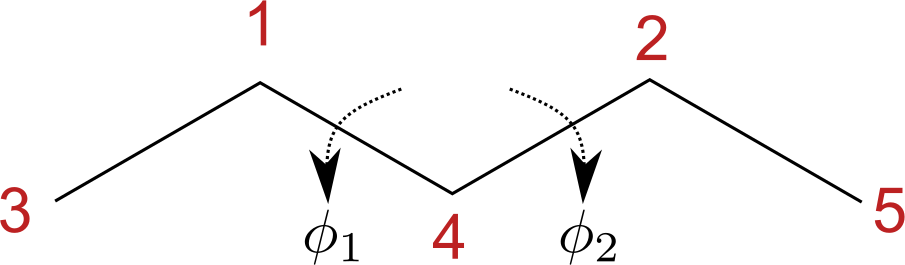
\includegraphics[width=.3\textwidth]{pentane}
  \caption{United-atoms pentane molecule.}
  \label{fig:pentane}
\end{figure}

The input trajectory (\texttt{pe.xyz}) is also the same for both
examples, and it contains a single configuration of pentane in vacuum:

\begin{lstlisting}[language=gromacs]
5
dihedral scan frame
 C            36.2175140         2.8697201        13.5523708
 C            38.7301917         2.1817050        13.2514028
 C            36.7128127         3.7399489        14.7152958
 C            37.2739523         2.0533908        12.7853724
 C            39.6555292         1.3152352        12.3955582
\end{lstlisting}\vspace{2ex}\par

\noindent

\subsection{Based on a SPEC file}
\label{sec:tutorial-profilergen-spec}

The dihedral-angle specification file (\texttt{dih.spec}) for the
torsional-scan angles described above is a file containing the matrix
in \autoref{eq:tutorial-gen-matrix}, with each row in a line and with
the columns separated by blank characters.

To run the \profilergen{} job for pentane based on this SPEC file,
enter the appropriate directory

\begin{lstlisting}[language=bash]
$  cd doc/tutorial/profilerGen/spec
\end{lstlisting}\vspace{2ex}\par

\noindent
and run \profilergen{} using the appropriate STP, XYZ and SPEC files as input:

\begin{lstlisting}[language=bash]
$  profilerGen -c pe.xyz -t pe.stp -s dih.spec -op pe_spec -dk 5000
\end{lstlisting}\vspace{2ex}\par

\noindent
Notice that we used a single restraint force constant of
\SI{5000}{\kJ\per\mole\per\radian\squared} for both dihedrals, which
is compatible with listing both of them
under a single \texttt{[~refdihedrals~]} block.

The output files of this run are the XYZ trajectory file
\texttt{pe\_spec.xyz} and the DAT file \texttt{pe\_spec.dat}
containing the energy profile of the torsional scan. The energies are
listed in a ``flattened'' fashion, as a single column with $19^2$
rows, one for each torsional-scan configuration. When plotted as a
$19\times 19$ matrix using the corresponding values of $\phi_1$ and
$\phi_2$ as axes labels, the results is a nice-looking torsional PES,
as shown in \autoref{fig:pentane-pes}.

\begin{figure}[tb]
  \centering
  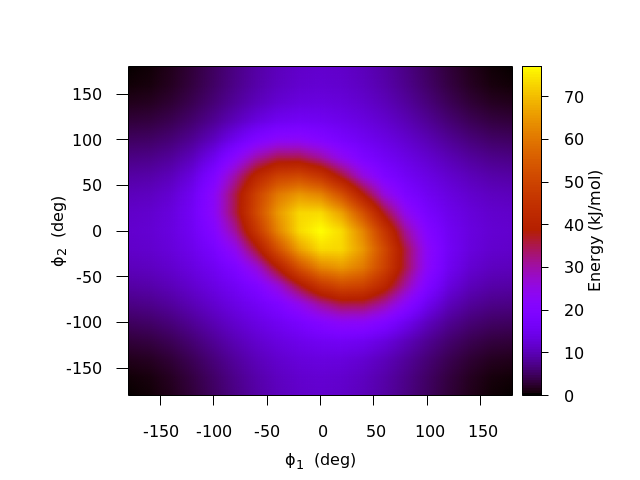
\includegraphics[width=.6\textwidth]{pe_spec}
  \caption{Torsional PES for pentane generated with \profilergen{}
    (see \autoref{fig:pentane} for the definition of $\phi_1$ and
    $\phi_2$).}
  \label{fig:pentane-pes}
\end{figure}

\subsection{Based on a Systematic Scan}
\label{sec:tutorial-profilergen-scan}

To run the \profilergen{} job for pentane based on a systematic scan
that is equivalent to the SPEC file in the previous section, enter the
appropriate directory

\begin{lstlisting}[language=bash]
$  cd doc/tutorial/profilerGen/systematic
\end{lstlisting}\vspace{2ex}\par

\noindent
and run \profilergen{} using the appropriate STP and XYZ files and the
appropriate command-line arguments as input:

\begin{lstlisting}[language=bash]
$  profilerGen -c pe.xyz -t pe.stp -op pe_systematic -dr -180 20 180 -dk 5000
\end{lstlisting}\vspace{2ex}\par

\noindent
Notice that we used a single set of restraint settings for both
dihedrals: a force constant of
\SI{5000}{\kJ\per\mole\per\radian\squared} (option \texttt{-dk}) and
torsional-scan angles (\textit{along each dimension}) from
\SI{-180}{\degree} to \SI{180}{\degree} with a step of
\SI{20}{\degree} (option \texttt{-dr}).  This is compatible with
listing $\phi_1$ and
$\phi_2$ under a single \texttt{[~refdihedrals~]} block.

The output files of this run are the XYZ trajectory file
\texttt{pe\_systematic.xyz} and the DAT file \texttt{pe\_systematic.dat}
containing the energy profile of the torsional scan. The energies are
listed in a ``flattened'' fashion, as a single column with $19^2$
rows, one for each torsional-scan configuration. When plotted as a
$19\times 19$ matrix using the corresponding values of $\phi_1$ and
$\phi_2$ as axes labels, the results is a nice-looking torsional PES,
as shown in \autoref{fig:pentane-pes}.

\section{Optimizing the Parameters}
\label{sec:tutorial-profileropt}

The files for this part of the tutorial are in \texttt{./doc/tutorial/profilerOpt}.
They are split into two subdirectories: \texttt{atoms} and \texttt{pairs}.
The \texttt{atoms} subdirectory contains the files for a \profileropt{} run in which
the Lennard-Jones optimization is performed on the CH2 and CH3 atomtypes.
The \texttt{pairs} subdirectory contains the files for a \profileropt{} run in which
the Lennard-Jones optimization is performed on the CH2-CH3 and CH3-CH3 pairtypes.

The systems considered in this example are a united-atoms butane and a
united-atoms pentane molecule, with one reference dihedral each (see
\autoref{fig:tutorial-butane-pentane}).  The dihedral angle 5-2-4-1 of
the pentane molecule was not chosen as a reference dihedral because the
quantum-mechanical data for this molecule corresponds to a 1D scan along
the 3-1-4-2 dihedral angle.
%

Our intention is to derive a torsional potential that apply to all
dihedral angles, including the 5-2-4-1 dihedral angle of pentane,
together with 1--4 Lennard-Jones parameters that applies to all 1--4
pairs.
%
There are two ways to address the optimization of the Lennard-Jones
terms: the CH2-CH3 and CH3-CH3 pairtypes can be optimized explicitly
or atomic 1--4 terms can be optimized for the CH2 and CH3 atomtypes,
from which the pair parameters are derived \textit{via} mixing rule.
%

\begin{figure}[tb]
  \centering
  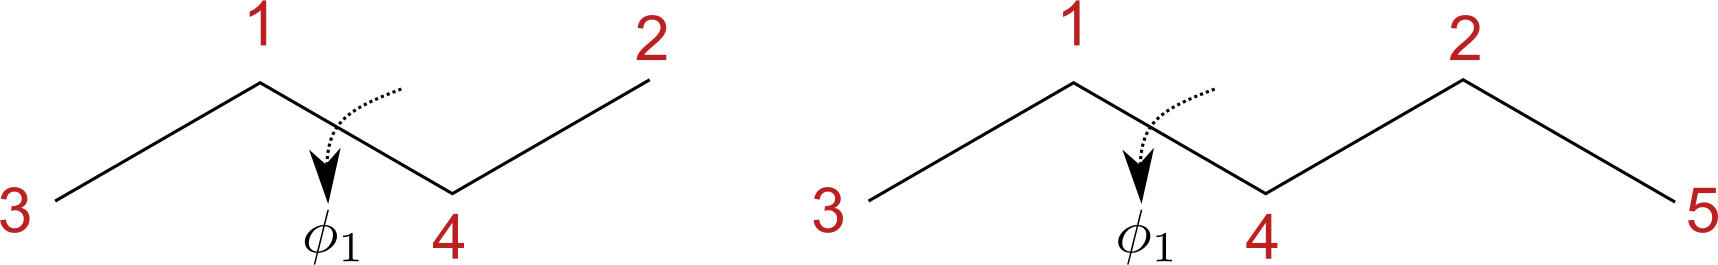
\includegraphics[width=0.6\textwidth]{butane_pentane}
  \caption{United-atoms butane and united-atoms pentane molecules.}
  \label{fig:tutorial-butane-pentane}
\end{figure}

\subsection{Understanding the Input-Parameters (INP) File}
\label{sec:tutorial-profileropt-inp}

When compared to \profilergen{}, \profileropt{} introduces a new input
file (the INP file) where the settings of the parameter optimization
are configured.
%
A complete description of the syntax of the INP file is available in
\autoref{sec:file-formats-INP}.
%
In this section, we briefly go over the contents of the INP file used
in this part of the tutorial.
%
The files for both examples
(\texttt{tutorial/profilerOpt/atoms/run.inp} and
\texttt{tutorial/profilerOpt/pairs/run.inp}) are the same, so any of
them can be used for this purpose.

The first block of the INP files is

\begin{lstlisting}[language=gromacs]
[ parameter_optimization ]
; NTORS   NLJ    FTORS
      1     2        1
; TORSNT
      0     0     2     0     0     0
; LJNT
      1   1
      1   1
; WTEMP
0
\end{lstlisting}\vspace{2ex}\par

\noindent
NTORS controls the number of optimized torsional types.
\varset{NTORS}{1} means that a single torsional type is optimized.
NLJ controls the number of optimized Lennard-Jones types.
\varset{NLJ}{2} means that two Lennard-Jones types are optimized (one
for each pair or one for each atom, depending on the example).  FTORS
controls the functional form of the torsional type in optimization.
\varset{FTORS}{1} means that the functional form is the standard
periodic one (\autoref{eq:proper-standard-energy}).  The matrix
TORSNT, with NTORS rows and 6 columns, controls which summands of the
torsional potential energy function are considered for each torsional
type, and also whether to optimize only the force constant or also the
phase.  It is set such that only the term with multiplicity 3 is used
in the torsional type, optimizing both the force constant and the
phase.  The matrix LJNT, with NLJ rows and 2 columns, controls which
components of the Lennard-Jones potential are optimized for each
Lennard-Jones type. It is set such that both the attractive and
repulsive components are optimized, for both types. WTEMP is the
temperature used for Boltzmann-weighting of the reference data.
\varset{WTEMP}{0} actually means an infinite temperature, which is
equivalent to setting all weights to 1.

The second block is

\begin{lstlisting}[language=gromacs]
[ parameter_randomization ]
; PINV
    50
; DIST[I]  MIN[I]    MAX[I]     MEAN[I]  STDDEV[I]
        2       0        30        20.0        8.0
        2       0         1        8e-3      24e-3
        2       0         1        8e-6      24e-6
\end{lstlisting}\vspace{2ex}\par

\noindent and contains the details of the obtention of random
parameters.
%
The distributions (DIST) from which torsional, $CS_6$ and $CS_{12}$
values are drawn, respectively, are specified along with their mean
(MEAN), standard deviation (STDDEV) and minimum (MIN) and maximum
allowed (MAX) values.
%
All of these distributions are LogNormal.
%
In the case of torsional parameters, after randomly obtained, they may
have their sign reversed with a probability of 0.50 (PINV).

The third block is

\begin{lstlisting}[language=gromacs]
[ evolutionary_strat ]
; STRAT
      1
; POPSIZE    NGENS  
       50       50
\end{lstlisting}\vspace{2ex}\par

\noindent and contains the specification of the evolutionary algorithm
used to perform the optimization.  \varset{STRAT}{1} sets the
algorithm to CMA-ES.  \varset{POPSIZE}{50} and \varset{NGENS}{50} set
the size of the population and the number of generations,
respectively, to 50. Note that it usually takes a larger number of
generations, with a larger population, to achieve convergence in the
results of a \profileropt{} job. The values in this example are merely
for the purpose of illustration.

The fourth block is

\begin{lstlisting}[language=gromacs]
[ seed ]
    1485
\end{lstlisting}\vspace{2ex}\par

\noindent and sets the RNG seed to 1485.

The fifth block is

\begin{lstlisting}[language=gromacs]
[ minimization ]
;   MALG     DX0  DXM  NMAX  DELE
       1    0.05  0.2  5000  1e-5
       1   0.001  0.1 10000  1e-9
\end{lstlisting}\vspace{2ex}\par

\noindent and contains the settings of the minimization algorithms.
They correspond to two steepest-descents algorithms (MALG) of
different precision (DELE) and duration (NMAX).
%
The first one refers to the routine minimization performed for every
individual; it runs for at most 5000 steps or until the energy
difference between successive steps is less than $1\times 10^{-5}$ kJ~mol$^{-1}$.
%
The second one refers to the final minimization performed only for the
optimal individual; it runs for at most 10000 steps or until the energy
difference between successive steps is less than 10$^{-9}$
kJ~mol$^{-1}$.
%

The last block is

\begin{lstlisting}[language=gromacs]
[ torsional_scan ]
;  NTSCAN
        1
;  NRESTR
        1
;   RFRST  RSTEP  RLST   RFCT
        0     10   360   5000
\end{lstlisting}\vspace{2ex}\par

\noindent and specifies the settings of the torsional scan.
\varset{NTSCAN}{1} means that the torsional-scan angles are generated
by the program based on a multidimensional systematic scan.
\varset{NRESTR}{1} means that a single set of dihedral-restraint
settings is specified.  Note that NRESTR \textit{must be equal} to the
number of reference-dihedral groups in \textit{each and all} of the
STP files provided to \profileropt{}. The NRESTR following uncommented
lines specify the torsional-scan angles (RFRST, RSTEP and RLST) and
force-constant (RFCT) that apply to all the dihedrals of each
reference-dihedral group.  RFRST, RSTEP and RLST are ignored if the
torsional-scan angles originate from an external source (for example,
from a SPEC file).  The molecules considered in this example have only
one reference-dihedral group, with one dihedral angle that is
restrained to the values
$(\SI{0}{\degree},\SI{10}{\degree},\ldots,\SI{360}{\degree})$ using a
force constant of \SI{5000}{\kJ\per\mole\per\radian\squared}.

\subsection{Optimizing Atomtypes}
\label{sec:tutorial-profileropt-atoms}

To carry out the optimization, it is necessary to specify the atom
indexes of the reference dihedrals and of the optimized dihedral
angles and atomtypes.
%
This is done in the STP files
\texttt{./doc/tutorial/profilerGen/atoms/bu.stp} and
\texttt{./doc/tutorial/profilerGen/atoms/pe.stp}, together with the
specification of the topology itself.
%
For butane and pentane, the reference dihedral $\phi_1$ is

\begin{lstlisting}[language=gromacs]
[ refdihedrals ]
; idx
3   1   4   2
\end{lstlisting}\vspace{2ex}\par

The optimized atomtypes are a bit more trickier to specify.
If the atomtypes are $(\text{CH2}, \text{CH3})$, then butane has no atoms
of the first atomtype and two atoms of the second atomtype: 2 and 3.
This is indicated in the STP file by

\begin{lstlisting}[language=gromacs]
[ optatoms ]
; CH2 - empty

[ optatoms ]
; CH3
2   3
\end{lstlisting}\vspace{2ex}\par

\noindent Analogously, for pentane, we have:

\begin{lstlisting}[language=gromacs]
[ optatoms ]
; CH2
1    2    4

[ optatoms ]
; CH3
3    5
\end{lstlisting}\vspace{2ex}\par

The optimized dihedral angle for butane is obvious:

\begin{lstlisting}[language=gromacs]
[ optdihedrals ]
; idxs
3   1   4   2   
\end{lstlisting}\vspace{2ex}\par

\noindent{}
The optimized dihedral angles for pentane are \textit{both} 3-1-4-2
and 5-2-4-1.
%
They are listed in the same \texttt{[~optdihedrals~]} block, since
they are modelled by the same torsional type:

\begin{lstlisting}[language=gromacs]
[ optdihedrals ]
    3    1    4    2
    5	 2    4	   1
\end{lstlisting}\vspace{2ex}\par

Contrary to \profilergen{}, \profileropt{} requires complete
torsional-scan trajectories as input. The trajectories
\texttt{./doc/tutorial/profilerOpt/atoms/bu.xyz} (of butane) and
\texttt{./doc/tutorial/profilerOpt/atoms/pe.xyz} (of pentane) consist
of 37 configurations where the reference torsional-scan dihedral angle
assumes, in turn, the values
$(\SI{0}{\degree}, \SI{10}{\degree}, \ldots, \SI{360}{\degree})$.
These input trajectories can be obtained with \profilergen{}, as
illustrated in \autoref{sec:tutorial-profilergen}.

The reference energy values for the optimization can be found in the
files \texttt{bu.dat} (of butane) and \texttt{pe.dat} (of pentane) in
the subdirectory \texttt{./doc/tutorial/profilerOpt/atoms}. They were
obtained from quantum-mechanical dihedral scans along the reference
dihedrals, using settings that match the torsional-scan settings
specified in the INP file (see
\autoref{sec:tutorial-profileropt-inp}).

To run the \profileropt{} job, enter the appropriate directory

\begin{lstlisting}[language=bash]
$  cd doc/tutorial/profilerOpt/atoms
\end{lstlisting}\vspace{2ex}\par

\noindent
and run \profileropt{} using the appropriate input files and 
command-line arguments:

\begin{lstlisting}[language=bash]
$  profilerOpt -np 8 -r bu.dat pe.dat -c bu.xyz pe.xyz -t bu.stp pe.stp -i run.inp -op atomic
\end{lstlisting}\vspace{2ex}\par

\noindent
The job is parallelized across 8 processors for the sake of speed.
This number can be incremented or decremented depending on the machine
in which you are following this tutorial.

As indicated in \autoref{sec:program-opt}, a successful run of
\profileropt{} will create several output files of which the formats
are described in \autoref{sec:file-formats-file-formats}.
%
For the sake of thoroughness, we will comment on each of these output
files and the interpretation of their contents.
%
The IFP file (\texttt{atomic.ifp}) reads

\begin{lstlisting}[language=gromacs]
Type 0
     cs6 = 2.8126163e-04     
    cs12 = 1.6387810e-06     
Type 1
     cs6 = 3.0038972e-03     
    cs12 = 3.1436281e-06     
Type 2
       k_3 = -7.0104044e+00    
     phi_3 = -1.8001386e+02    
rmsd = 0.4175188710494903
\end{lstlisting}\vspace{2ex}\par

\noindent
and contain the main results of the parameter optimization.  The last
line contains the value of the WRMSD (in \si{\kJ\per\mole}) for the
best individual.  The lines above list the optimized parameter values
for each parameter type.  The first parameters are those of the
Lennard-Jones types, in the order they are defined in the STP and INP
files.  Therefore, in this case, type 0 applies to the CH2 atomtype,
while type 1 applies to the CH3 atomtype.  After that, the parameters
of the torsional types are listed, also in the order they are defined
in the STP and INP files.  Therefore, in this case, type 2 is the
single torsional type defined in this example. The subscripts in the
torsional parameters indicate the summand of the torsional potential
function\textemdash{}in this case, the optimized parameters are the
force constant and the phase of the term with multiplicity 3.

The energy profiles for the best individual are listed for two
different energy-minimization settings. The files
\texttt{atomic\_1.dat} and \texttt{atomic\_2.dat} contain the energy
profiles considered during the execution of the evolutionary
algorithm.  The order of the systems follows the order their files
were written in the command-line arguments: first butane, then
pentane. Each DAT file has a single-column and a number of rows equal
to the length of the torsional scan\textemdash{}in this case, 37 data
points. The value in the $k$-th row is the energy of the $k$-th
configuration of the torsional scan (see \autoref{sec:ga-tpes}).  The
files \texttt{atomic\_minim\_1.dat} and \texttt{atomic\_minim\_2.dat}
follow the same structure, but contain refined energy values obtained
after re-running the torsional scan of the optimal individual with
enhanced energy-minimization settings (see the explanation of the
\texttt{[~minimization~]} block in
\autoref{sec:tutorial-profileropt-inp}). These energy profiles are
plotted together with the reference data (\texttt{bu.dat} and
\texttt{pe.dat}) in \autoref{fig:tutorial-profileropt-results}.  In
this case, the results for the original and enhanced
energy-minimization settings are almost indistinguishable.  Note that,
for comparison, the reference data was subtracted by its average value
for each molecule.

\begin{figure}[tb]
  \centering
  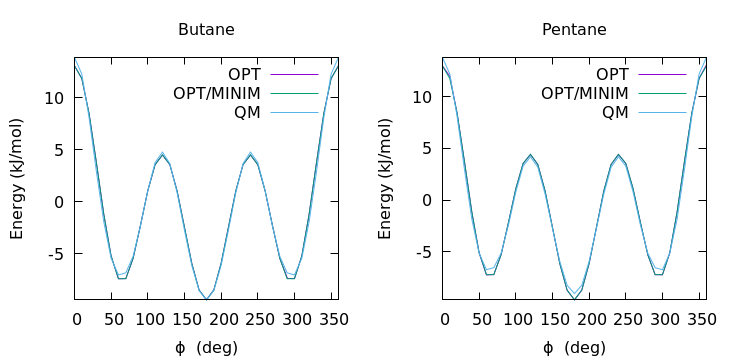
\includegraphics[width=.8\textwidth]{opt-results}
  \caption{Optimization results for butane and pentane.}
  \label{fig:tutorial-profileropt-results}
\end{figure}

The XYZ files \texttt{atomic\_1.xyz}, \texttt{atomic\_2.xyz},
\texttt{atomic\_minim\_1.xyz} and \texttt{atomic\_minim\_2.xyz} are
the torsional-scan trajectories corresponding to the energy profiles
described above. In these files, the $k$-th frame is the configuration
of the $k$-th step of the torsional scan.

\subsection{Optimizing Pairtypes}
\label{sec:tutorial-profileropt-pairs}

The files for this part of the tutorial are in
\texttt{./doc/tutorial/profilerOpt/pairs}.  To perform the
optimization based on pairtypes instead of atomtypes (as in the
previous section), only one change is necessary.  Instead of
associating the two Lennard-Jones types under optimization to the CH2
and CH3 atoms, we now must associate them to the CH2-CH3 and CH3-CH3
pairs.  In practice, this is done by replacing the
\texttt{[~optatoms~]} blocks in the STP files by \texttt{[~optpairs~]}
blocks that convey this information. There will be two such blocks per
molecule, one for each pairtype. In \texttt{bu.stp}
(see \autoref{fig:tutorial-butane-pentane}):

\begin{lstlisting}[language=gromacs]
[ optpairs ]
; CH2-CH3 empty

[ optpairs ]
; CH3-CH3
2   3
\end{lstlisting}\vspace{2ex}\par

\noindent In \texttt{pe.stp}
(see \autoref{fig:tutorial-butane-pentane}):

\begin{lstlisting}[language=gromacs]
[ optpairs ]
; CH2-CH3
1   5
2   3

[ optpairs ]
; CH3-CH3 - empty
\end{lstlisting}\vspace{2ex}\par

Apart from this difference in the STP files, the optimization of
pairtypes follows the same steps as the optimization of atomtypes
described in the previous section.
%
To run the \profileropt{} job, enter the appropriate directory

\begin{lstlisting}[language=bash]
$  cd doc/tutorial/profilerOpt/pairs
\end{lstlisting}\vspace{2ex}\par

\noindent
and run \profileropt{} using the appropriate input files and 
command-line arguments:

\begin{lstlisting}[language=bash]
$  profilerOpt -np 8 -r bu.dat pe.dat -c bu.xyz pe.xyz -t bu.stp pe.stp -i run.inp -op pairs
\end{lstlisting}\vspace{2ex}\par

The optimized parameters are in the IFP file (\texttt{pairs.ifp}):

\begin{lstlisting}[language=gromacs]
Type 0
     cs6 = 1.6450521e-04     
    cs12 = 1.9323756e-06     
Type 1
     cs6 = 2.6969757e-03     
    cs12 = 2.9638616e-06     
Type 2
       k_3 = -7.0186282e+00    
     phi_3 = -1.8023863e+02    
rmsd = 0.4188594022812412
\end{lstlisting}\vspace{2ex}\par

\noindent
The torsional parameters are essentially the same to those obtained in
the optimization of atomtypes.  The Lennard-Jones parameters, however,
are slightly different (even after applying the geometric mixing
rule). In spite of that, the energy profiles are almost
indistinguishable, as indicated by the WRMSD values (difference is
less than \SI{1e-2}{\kJ\per\mole}).

For a complete description of the output files, see the previous
section.

\begin{thebibliography}{9}
  \bibitem{DEAP}
    Fortin, F., Fran\c{c}ois-Michel De Rainville, Gardner, M., Parizeau, M. and Gagn\'e, C. DEAP: evolutionary algorithms made easy. Journal of Machine Learning Research, 13, 2171–2175 (2012). 
\bibitem{GROMOS-doc} van Gunsteren, W. F., Billeter, S. R., Eising,
  A. A., Hünenberger, P. H., Krüger, P., Mark, A. E., Scott,
  W. R. P. and Tironi, I. G. Biomolecular Simulation: The GROMOS96
  Manual and User Guide. Volume~2:~Algorithms and Formulae for
  Modelling of Molecular Systems, Vdf Hochschulverlag AG an der ETH
  Zürich, Zürich, Switzerland, 1996.
\bibitem{GROMACS-doc} Abraham, M.~J., van~der~Spoel, D., Lindahl,~E.,
  Hess,~B. and the GROMACS development team. GROMACS User Manual
  version 2019. \url{http://www.gromacs.org}.
\end{thebibliography}

\appendix
\chapter{MIT License}
\label{appendix:MIT-license}

\begin{verbatim}
MIT License

Copyright (c) 2020 mssm-labmmol

Permission is hereby granted, free of charge, to any person obtaining a copy
of this software and associated documentation files (the "Software"), to deal
in the Software without restriction, including without limitation the rights
to use, copy, modify, merge, publish, distribute, sublicense, and/or sell
copies of the Software, and to permit persons to whom the Software is
furnished to do so, subject to the following conditions:

The above copyright notice and this permission notice shall be included in all
copies or substantial portions of the Software.

THE SOFTWARE IS PROVIDED "AS IS", WITHOUT WARRANTY OF ANY KIND, EXPRESS OR
IMPLIED, INCLUDING BUT NOT LIMITED TO THE WARRANTIES OF MERCHANTABILITY,
FITNESS FOR A PARTICULAR PURPOSE AND NONINFRINGEMENT. IN NO EVENT SHALL THE
AUTHORS OR COPYRIGHT HOLDERS BE LIABLE FOR ANY CLAIM, DAMAGES OR OTHER
LIABILITY, WHETHER IN AN ACTION OF CONTRACT, TORT OR OTHERWISE, ARISING FROM,
OUT OF OR IN CONNECTION WITH THE SOFTWARE OR THE USE OR OTHER DEALINGS IN THE
SOFTWARE.
\end{verbatim}

\end{document}
